\documentclass[11pt,a4paper]{article}

\usepackage{geometry}
\geometry{legalpaper, margin=1in}

\usepackage[utf8]{inputenc}
\usepackage[T1]{fontenc}
\usepackage{amsmath,amssymb,amsfonts}
\usepackage{graphicx}
\usepackage{float}
\usepackage{hyperref}
\usepackage{xcolor}
\usepackage{caption}
\usepackage{subcaption}
\usepackage{amsmath, amssymb}
\usepackage{graphicx}
\usepackage{booktabs}
\usepackage{tcolorbox}
\usepackage{fontawesome5} % for icons
\usepackage{enumitem}


\title{Methods in Computational Neuroscience\\
Ring Attractor Network (Noorman et al., 2024)}
\author{Sepehr Saeedpour}
\date{June 2025}

\begin{document}

\maketitle

\section*{Introduction}
Ring attractor networks provide a foundational computational framework for representing circular, continuous variables such as head direction, spatial orientation, or phase information by sustaining a localized "bump" of persistent neural activity. These activity bumps can stably occupy any position along a one-dimensional ring manifold, forming a continuum of marginally stable fixed points. This property emerges from a "Mexican-hat" connectivity profile characterized by sharp local excitation balanced against broader inhibition, effectively flattening the network's energy landscape. As a result, even infinitesimal velocity inputs can smoothly shift the bump without drift.

Classical theoretical analyses, developed for networks in the large-N limit, predict that an ideally flat manifold, and thus near-perfect precision, requires large neuron counts. With fewer neurons, this ring manifold was traditionally expected to fragment into discrete attractor states, causing the emergence of preferred orientations, spontaneous drift, and velocity integration thresholds. Consequently, classical theory suggests a direct trade-off between network size and discretization errors, implying biological circuits must be large to achieve accurate continuous dynamics.

Recent electron microscopy reconstructions of compass neurons in Drosophila melanogaster challenge this perspective. These studies have shown that the fly's head-direction system comprises remarkably few computational units, far fewer than classical models would suggest necessary. Complementary two-photon calcium imaging further reveals that this minimal network can nonetheless maintain a smoothly rotating activity bump that accurately tracks the fly's head direction in darkness, exhibiting negligible drift and no clear discretized orientations. These empirical findings demonstrate that biologically accurate continuous attractors can be achieved with surprising neuronal economy.

Inspired by these results, Noorman et al. (2024) constructed a threshold-linear ring attractor model with just six neurons. They analytically demonstrated that by fine-tuning local excitation to one of several discrete "sweet-spot" values, the curvature of the network's energy landscape can be reduced to zero. This effectively creates a seamless ring composed of multiple interconnected line attractors, resulting in marginally stable states. Numerical simulations confirmed that these networks could sustain drift-free persistent activity and perform linear integration of velocity inputs, even at arbitrarily small magnitudes.

This validates these theoretical predictions through systematic analysis of ring attractor dynamics across parameter spaces and network sizes. 
Using Principal Component Analysis (PCA) to visualize the geometry of attractor manifolds, we confirmed that optimal excitation tuning produces smooth ring manifolds, while deviations create either discrete point attractors or unstable dynamics. 
Crucially, we demonstrate that network size fundamentally affects parameter sensitivity: while small networks require precise tuning to maintain continuous dynamics, larger networks (N=100) exhibit robust continuous attractors across broader parameter ranges. '
Additionally, we show that feedforward input is essential for stable bump positioning, and that external velocity inputs can drive smooth motion along optimally tuned ring manifolds. 
These findings provide a strong support for the biological plausibility of minimal yet sophisticated neural circuits capable of continuous variable representation, with important implications for understanding navigation systems in compact brains.


\begin{tcolorbox}[
    enhanced,
    colback=gray!10,
    colframe=gray!50!black,
    title={\faBook\ Glossary},
    fonttitle=\bfseries\large,
    attach boxed title to top left={yshift=-3mm,xshift=5mm},
    boxed title style={
        colback=gray!50!black,
        coltext=white,
        rounded corners
    },
    boxrule=1pt,
    rounded corners,
    drop shadow,
    left=8pt,
    right=8pt,
    top=8pt,
    bottom=8pt
]
\begin{description}[leftmargin=0pt, labelsep=1em, itemsep=0.5em]
    \item[\textcolor{blue}{\textbf{Energy landscape}}]%
        A scalar “height-map’’ \(E(\mathbf{x}) = E(x_{1},\dots,x_{n})\) that gives every network state one energy value. 
        Valleys where \(\nabla_{\!\mathbf{x}}E = \mathbf{0}\) are stable; passes are saddles. 
        Near a minimum \(\mathbf{x}^{*}\),
        \[
        E(\mathbf{x}) \;\approx\; E(\mathbf{x}^{*}) + \tfrac12(\mathbf{x}-\mathbf{x}^{*})^{\!\top}\mathbf{H}(\mathbf{x}-\mathbf{x}^{*}),
        \quad
        H_{ij} = \Bigl.\dfrac{\partial^{2}E}{\partial x_{i}\partial x_{j}}\Bigr|_{\mathbf{x}^{*}} ,
        \]
        so positive Hessian eigenvalues ensure stability, while tiny ones mark “flat’’ directions.
        In Noorman \emph{et al.} the landscape \(E(a,w,\psi;J_E,J_I)\) for bump amplitude \(a\), width \(w\) and orientation \(\psi\) flattens along \(\psi\) at specific \(J_E\) values, yielding a ring of equally low minima.

    \item[\textcolor{blue}{\textbf{Continuous attractor network}}]%
        A recurrent network whose activity \(\mathbf{r}(t)\) obeys gradient flow
        \[
           \tau\,\dot{\mathbf{r}} = -\nabla_{\!\mathbf{r}}E(\mathbf{r}),
        \]
        producing a \emph{manifold} of fixed points
        \(
           \mathcal{M} = \{\mathbf{r} : \nabla_{\!\mathbf{r}}E = \mathbf{0}\}.
        \)
        Motion along \(\mathcal{M}\) is neutrally stable (\(\lambda=0\)); off-manifold perturbations relax back.
        Noorman \emph{et al.} show that even a 4-neuron ring network can realize such a continuous attractor when \(J_E\) is tuned optimally.

    \item[\textcolor{blue}{\textbf{Bump of activity}}]%
        A localized firing-rate profile over neurons ordered by their preferred angle \(\theta\); e.g.
        \[
           r(\theta,t)=a\,e^{\kappa\cos(\theta-\psi(t))}
           \quad\text{or}\quad
           r(\theta,t)=a\,e^{-\frac{(\theta-\psi(t))^{2}}{2w^{2}}}.
        \]
        Parameters \(a\) (height), \(w\) (width) and \(\psi\) (centre) fully describe the bump.
        Short-range excitation plus broad inhibition pin its shape, while shifting \(\psi\) moves the bump around the ring.
        In the fly “compass’’ studied by Noorman \emph{et al.}, this bump tracks head direction even in darkness.
\end{description}

\end{tcolorbox}

\section{Methods}
\subsection{Mathematical Framework}
The dynamics of neuron \( j \) in a velocity-driven ring attractor network are governed by:

\begin{equation}
\tau \frac{d h_j}{dt} = -h_j + \frac{1}{N} \sum_{k=1}^N \left( W^{\text{sym}}_{jk} + v_{\text{in}} W^{\text{asym}}_{jk} \right) \phi(h_k) + c_{\text{ff}},
\label{eq:ring_dynamics}
\end{equation}

where \(\phi(h)\) represents the threshold-linear activation function:
\[
\phi(h) = [h]_+ = \max(0, h).
\]

The network's connectivity structure consists of symmetric and asymmetric components:
\begin{align}
W^{\text{sym}}_{jk} &= J_I + J_E \cos(\theta_j - \theta_k), \\
W^{\text{asym}}_{jk} &= \sin(\theta_j - \theta_k).
\end{align}

The symmetric component combines uniform inhibition (\(J_I\)) with local excitation modulated by the neurons' preferred orientations, while the asymmetric component enables directional sensitivity and velocity integration. Tables 1 and 2 detail the functional roles of all parameters in this framework.

% where $\theta_i = 2\pi i/N$ represents the preferred direction of neuron $i$, $J_E$ and $J_I$ control excitatory and inhibitory coupling strengths, $J_{vel}$ determines velocity integration strength, and $\delta$ introduces phase shifts for directional selectivity.

\begin{table}[h!]
\centering
\begin{tabular}{@{}llp{9cm}@{}}
\toprule
\textbf{Symbol} & \textbf{Type} & \textbf{Description} \\
\midrule
\( h_j \) & variable & Total synaptic input (current) to neuron \( j \) \\
\( \phi(h) \) & function & Threshold-linear activation function: \( \phi(h) = \max(0, h) \) \\
\( \tau \) & parameter & Neural integration time constant (slower when large) \\
\( N \) & parameter & Total number of neurons arranged on a ring \\
\( \theta_j \) & parameter & Preferred orientation of neuron \( j \), uniformly distributed in \([0, 2\pi)\) \\
\( v_{\text{in}} \) & input & External angular velocity input to the network \\
\( c_{\text{ff}} \) & parameter & Constant feedforward bias input to all neurons \\
\( J_E \) & parameter & Strength of the \emph{tuned} (cosine) component of connectivity (local excitation) \\
\( J_I \) & parameter & Strength of the \emph{untuned} (uniform) component of connectivity (global inhibition) \\
% \( W^{\text{sym}}_{jk} \) & derived & Symmetric connectivity: \( J_I + J_E \cos(\theta_j - \theta_k) \) \\
% \( W^{\text{asym}}_{jk} \) & derived & Asymmetric (velocity-sensitive) connectivity: \( \sin(\theta_j - \theta_k) \) \\
\bottomrule
\end{tabular}
\caption{Variables and parameters used in Eq. 1 and the network structure.}
\end{table}


\begin{table}[h!]
\centering
\begin{tabular}{@{}lp{12cm}@{}}
\toprule
\textbf{Parameter} & \textbf{Effect on Network Dynamics} \\
\midrule
\( \tau \) & Governs the timescale of neural responses. Large \( \tau \): slower integration, more smoothing. Small \( \tau \): rapid but potentially unstable dynamics. \\
\( J_E \) & Controls the strength of local excitation. Must be sufficiently strong to generate a stable bump. Too low: no bump. Too high: narrow or unstable bump. \\
\( J_I \) & Controls global inhibition. Helps normalize activity across neurons, limits bump width, prevents runaway excitation. \\
\( v_{\text{in}} \) & Angular velocity input that biases bump motion. Positive or negative values move the bump CW or CCW around the ring. \\
\( c_{\text{ff}} \) & Background excitation to ensure enough baseline input. Influences overall bump amplitude and whether any neurons are active. \\
\bottomrule
\end{tabular}
\caption{Qualitative effects of key parameters on bump dynamics and attractor behavior.}
\end{table}

\subsection{Simulation and Example Network}

\subsubsection*{Simulation Procedure}

To investigate the attractor landscape of the ring network, we simulated its dynamics across a range of initial conditions and network parameters. 
For each parameter setting, the network’s architecture was defined by a symmetric weight matrix implementing local excitation and global inhibition, and an antisymmetric matrix representing velocity-modulated input. 
To probe the full range of attractor states, we initialized the network with 1000 distinct activity patterns, each corresponding to a cosine-shaped “bump” of activity centered at a different orientation $\psi$ around the ring.
Each initial state was constructed using the analytical bump formula from Eq. (S16) in the Supplementary Information of Noorman et al. (2024):

\begin{equation}
h_j^{(0)} = a \left[\cos(\theta_j - \psi) - \cos\left(\frac{w}{2}\right)\right]_+
\end{equation}


where $\theta_j = \frac{2\pi(j-1)}{N}$ is the preferred orientation of neuron $j$, $a$ is the bump amplitude, and $w$ is the bump width. This ensures the bump is centered at $\psi$ and spans a localized region on the ring.

The network dynamics were simulated over a time interval $T = 5.0\,\text{s}$ using the Euler–Maruyama  method with a fixed time step of $\Delta t = 0.01\,\text{s}$. For each initial condition, the system was numerically integrated until convergence to a fixed point. 
The resulting final activity vectors were recorded and collectively represent the attractor states of the network under the specified parameters.

\subsubsection*{Example Network}

We visualized the network connectivity and bump dynamics for a ring attractor model with $N = 6$ neurons, using parameters $J_E = 3.0$, $J_I = -1.0$, and $\tau = 0.1$ (Fig 1). 
The symmetric connectivity matrix $W^{\text{sym}}$ defines local excitation and broad inhibition via a cosine profile, while the asymmetric matrix $W^{\text{asym}}$ supports velocity-driven shifts in bump position. 
After simulating the network dynamics from a cosine-shaped initial condition, the system evolves to a persistent bump of activity. 
The support of this bump identifies a subset of active neurons, whose interactions define a principal submatrix of $W^{\text{sym}}$ ((Fig 1 Bottom)). 
This submatrix governs the local linear dynamics and plays a key role in determining the stability of the attractor.

\begin{figure}[htbp]
    \centering
    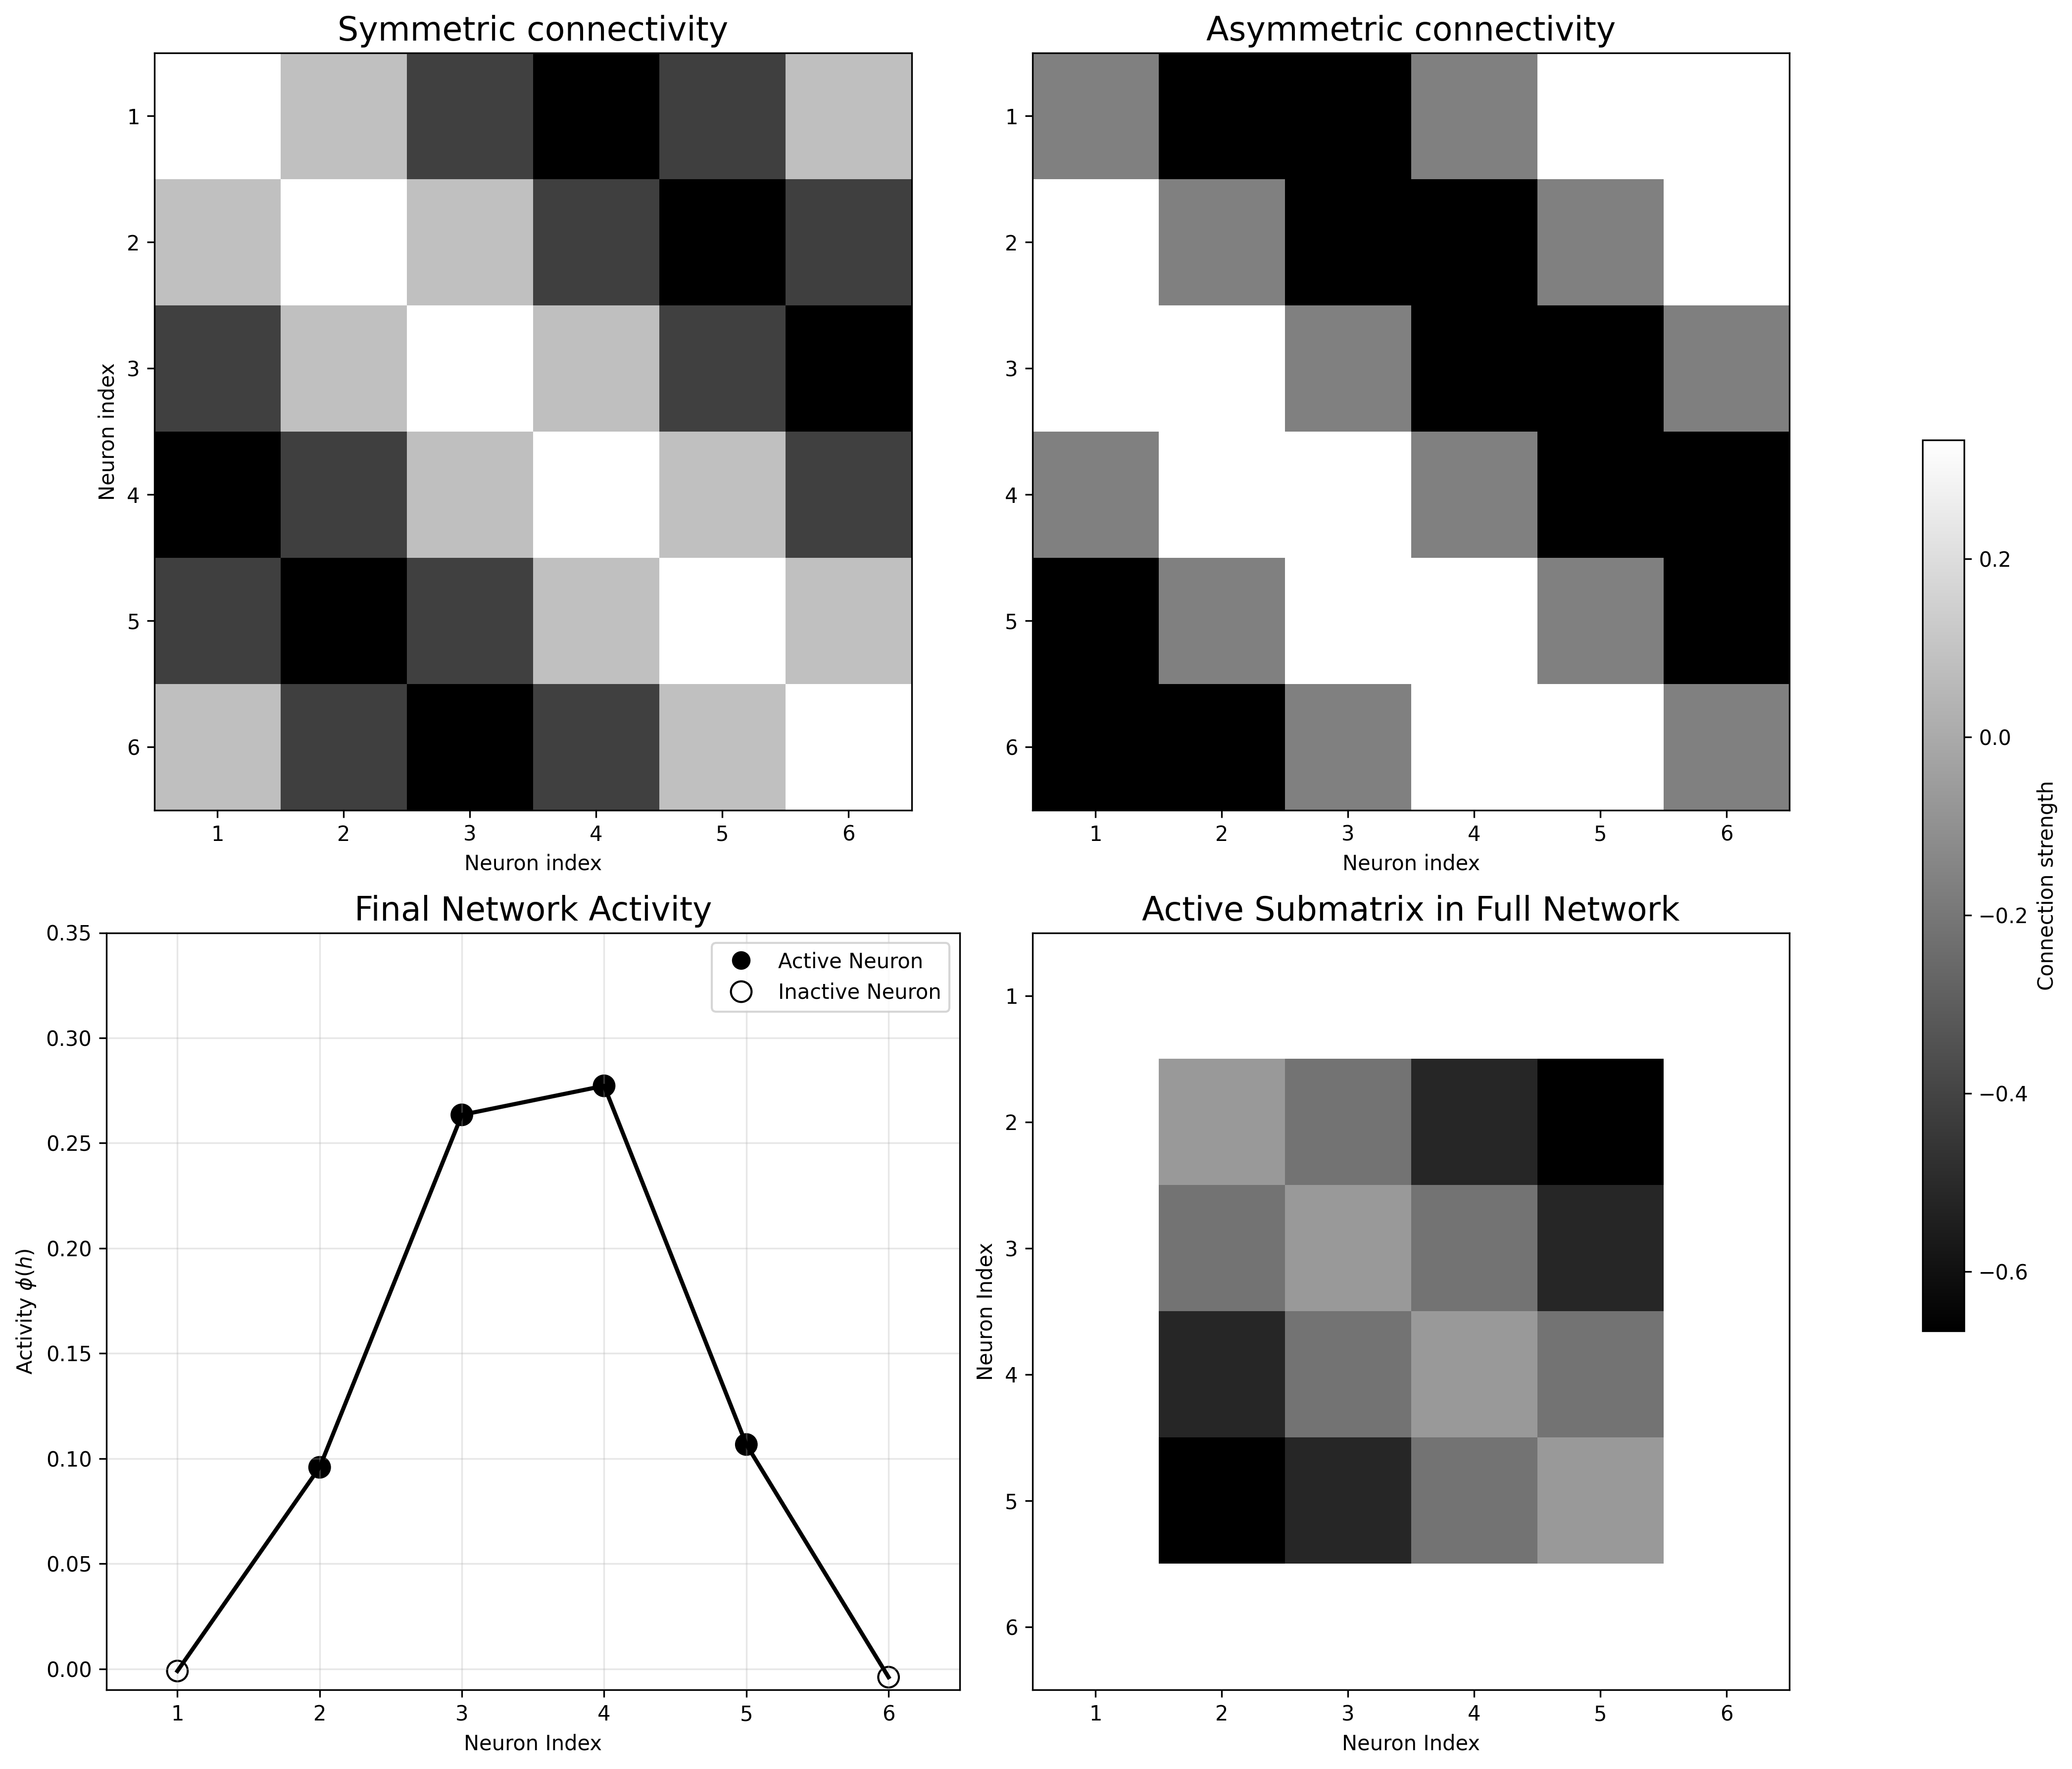
\includegraphics[width=0.8\textwidth]{connectivity_and_activity.png}
    \caption{Network structure and activity pattern of a 6-neuron ring attractor. \textbf{Top:} Symmetric weight matrix (left) implementing local excitation and global inhibition, and asymmetric weight matrix (right) for velocity integration. \textbf{Bottom:} Final network activity showing persistent bump with active neurons highlighted (left), and the corresponding submatrix of symmetric weights restricted to active neurons (right).}
    \label{fig:network_structure}
\end{figure}


\subsubsection*{PCA Analysis}

To analyze the structure of the network’s attractor dynamics, we applied Principal Component Analysis (PCA) to the population activity. We simulated a network of $N = 6$ neurons with parameters $J_I = -2.0$, $J_E = 4.0$, $v_{\text{in}} = 1.5$, and $c_{\text{ff}} = 1$, and recorded the full 6-dimensional neural activity across 1000 trials as the network encoded a continuously varying the orientation (Fig 2). 
We centered the activity data, computed the covariance matrix, and performed eigenvalue decomposition using \texttt{NumPy}. 



\section{Results}

\subsection{PCA results}

\subsubsection*{Manual vs. \texttt{scikit-learn} PCA}

To validate the robustness of our PCA-based analysis, we compared the results of our manual implementation with those obtained using the \texttt{scikit-learn} library. 
Both methods produced identical eigenvalues and a cosine similarity of 1 between corresponding principal components (components beyond the third are nearly zero), confirming the correctness of our implementation (Figure 2). Minor visual differences observed in Fig 2 are explained by the fact that PCA eigenvectors are only defined up to a sign; thus, some components appear flipped in direction, but still span the same subspace.




\subsubsection*{Low-Dimensional Ring Manifold}

Mapping the full neural state space onto the first three principal components reveals a pronounced ring manifold (Fig. 2 ).
Colour–coding each point by its underlying head-direction angle exhibits a one-to-one, circular correspondence between behaviour and network state. 
The mild ripples along the third component are not energy bumps; they arise from finite-size bump-shape fluctuations and the sign indeterminacy of PCA axes. 
So the manifold remains energetically flat and effectively two–dimensional, indicating that the chosen $J_E$ is close to the optimal value $J_E^{\ast}$ that ensures continuity. 
In the following section, we examines how different parameter sets influence this ring.


\begin{figure}[H]
\centering
\begin{subfigure}{0.24\textwidth}
    \centering
    \caption*{\textbf{A}}
    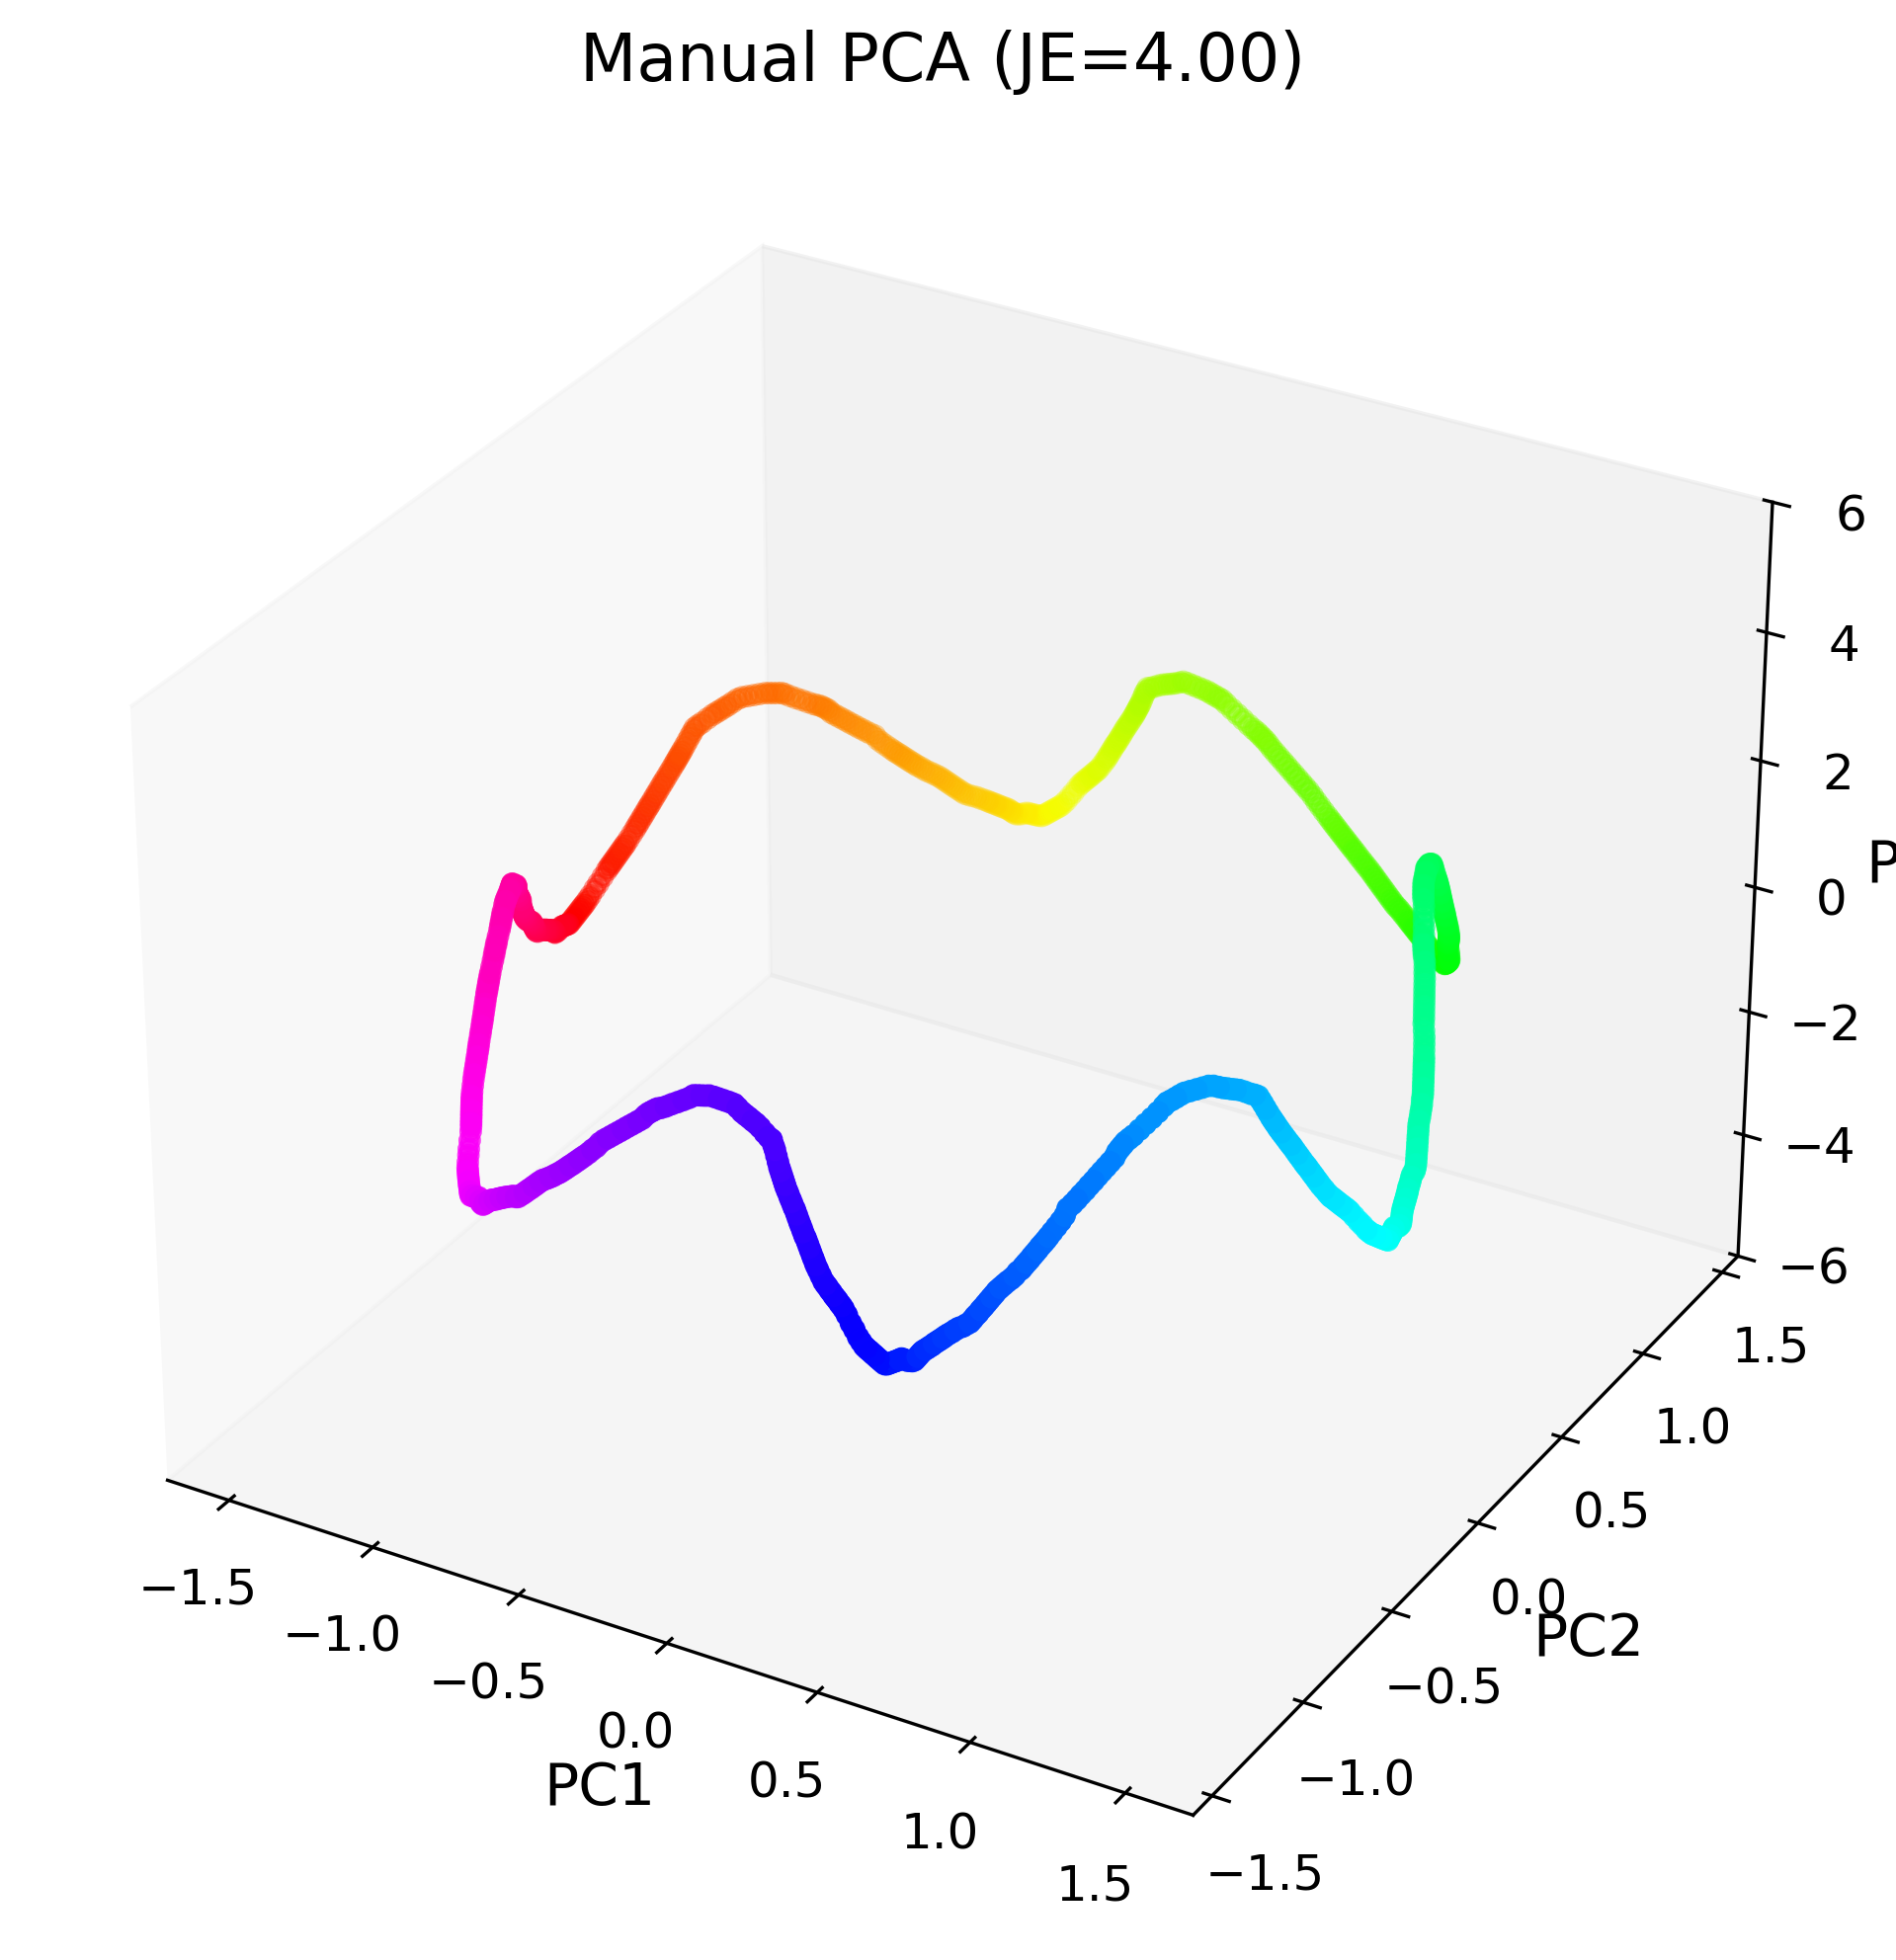
\includegraphics[width=\textwidth]{manual_pca.png}
\end{subfigure}
\hfill
\begin{subfigure}{0.24\textwidth}
    \centering
    \caption*{\textbf{B}}
    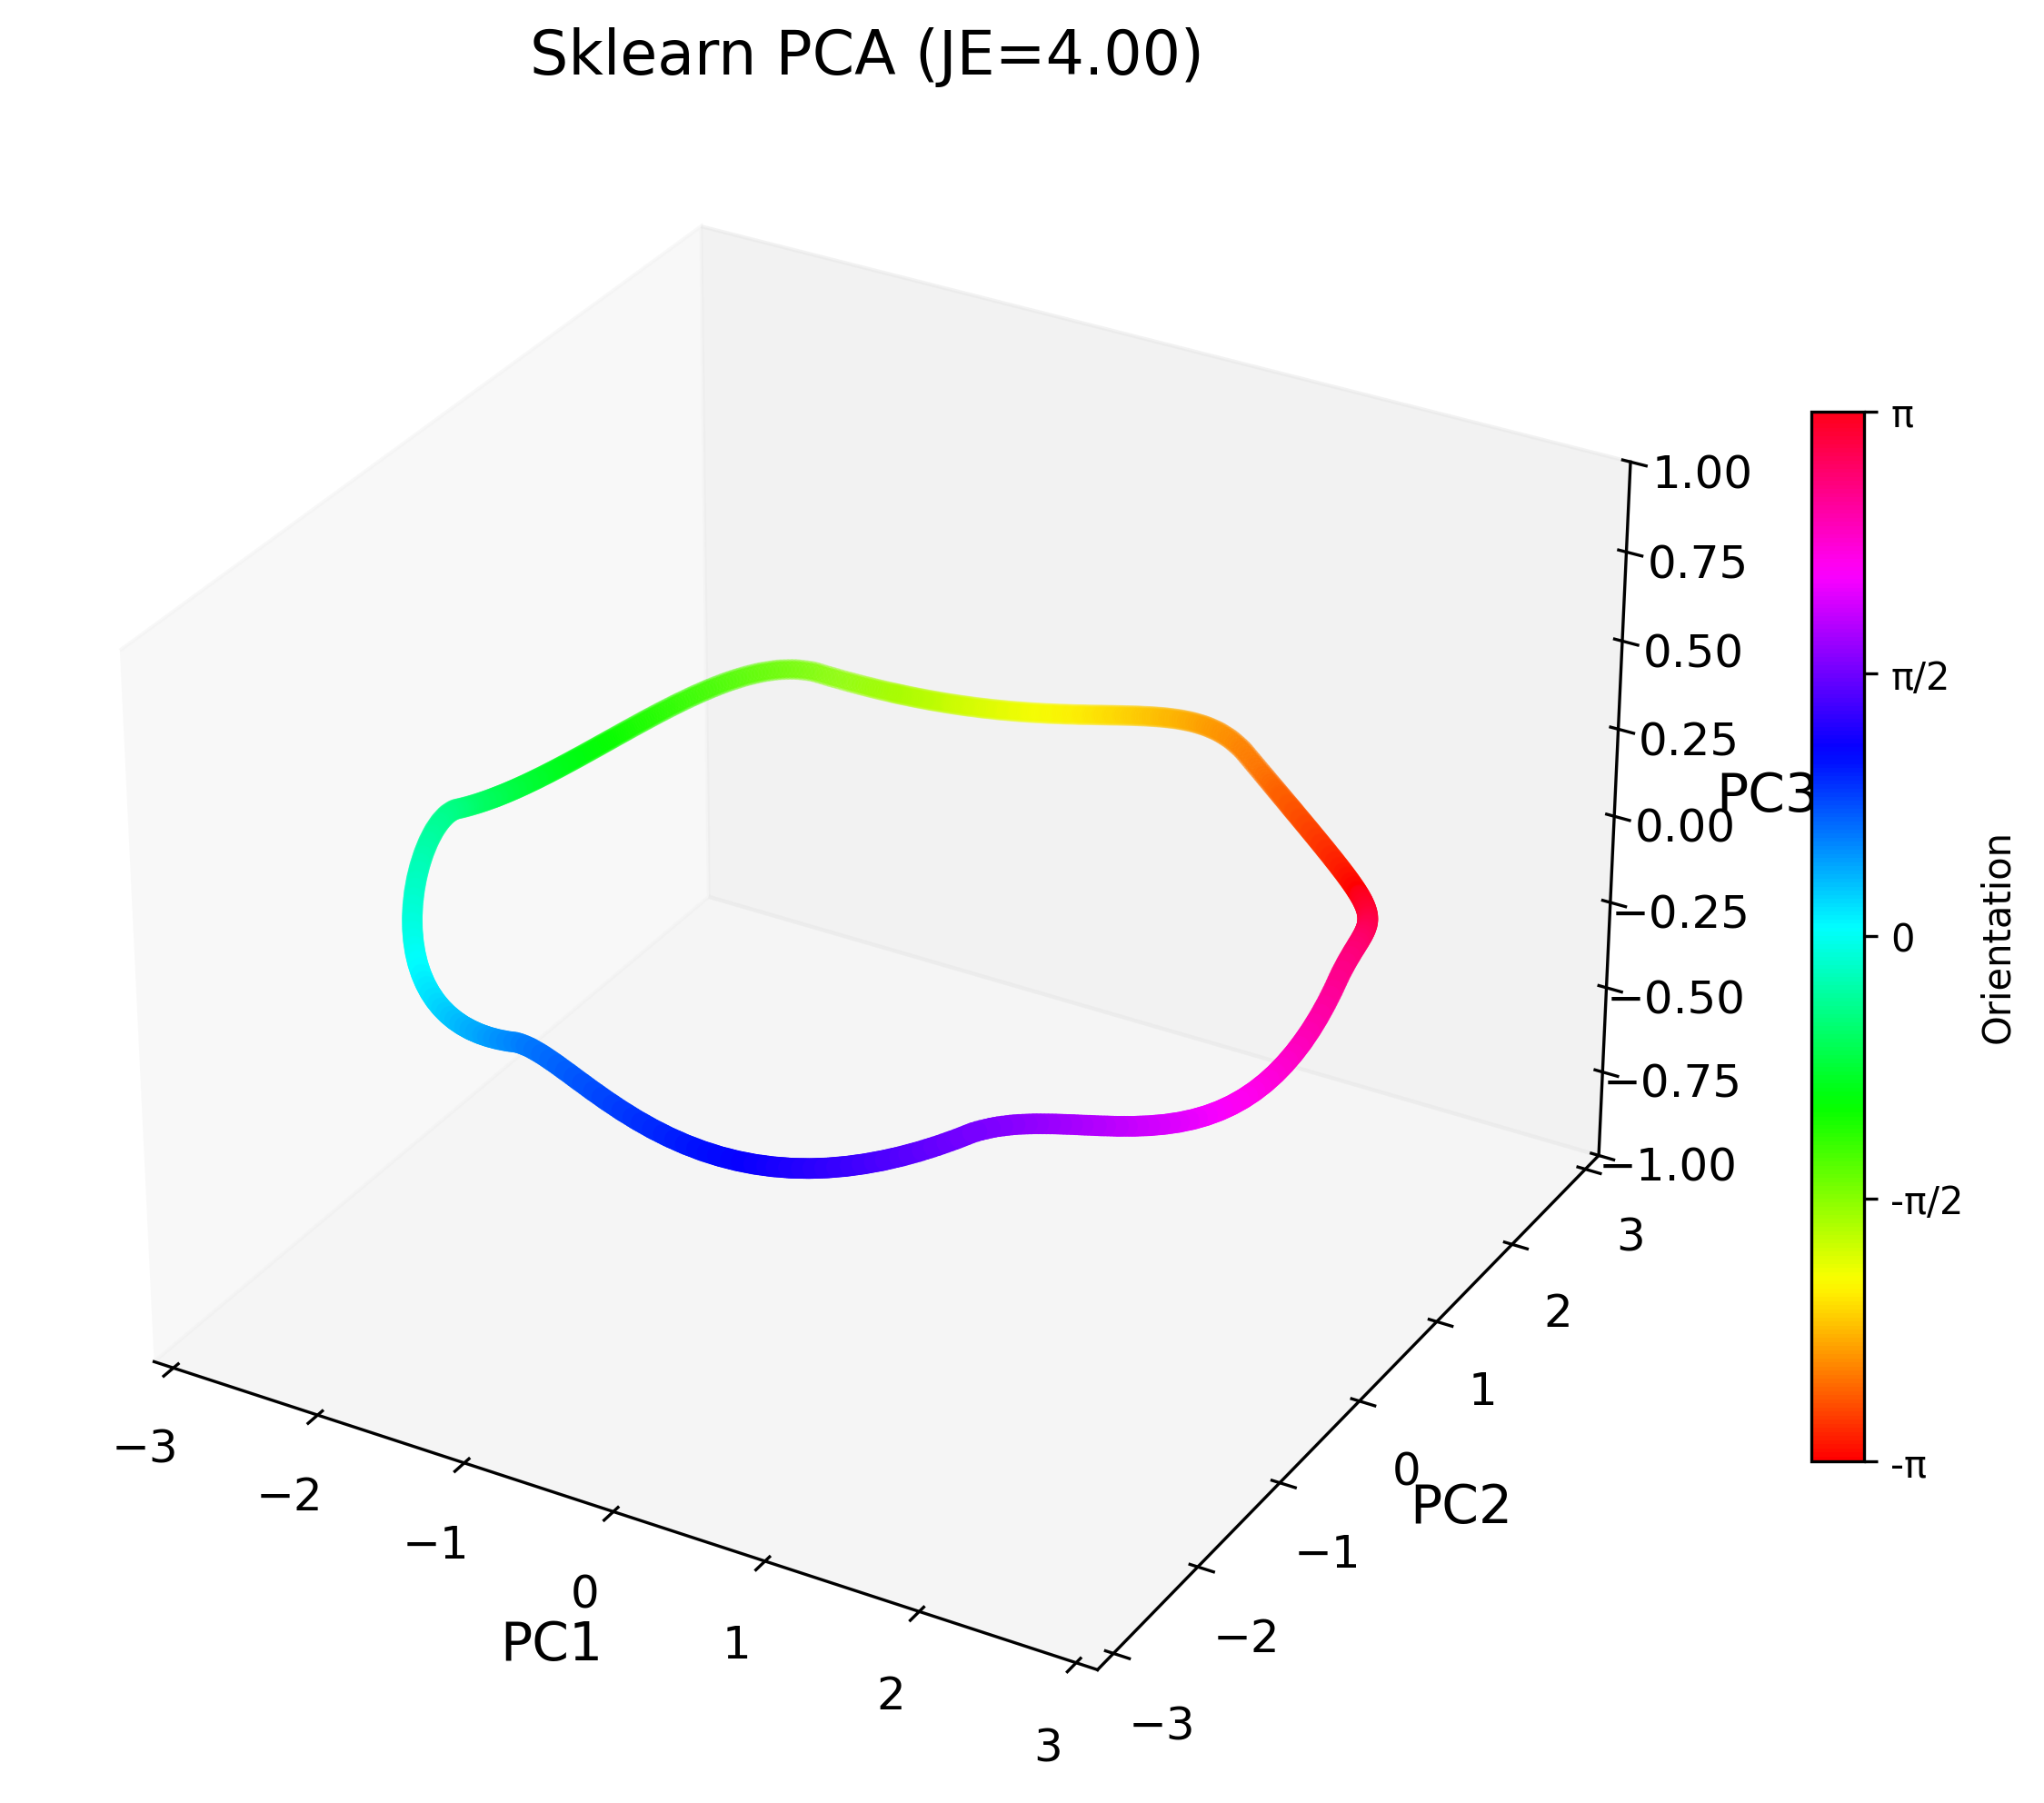
\includegraphics[width=\textwidth]{sklearn_pca.png}
\end{subfigure}
\hfill
\begin{subfigure}{0.24\textwidth}
    \centering
    \caption*{\textbf{C}}
    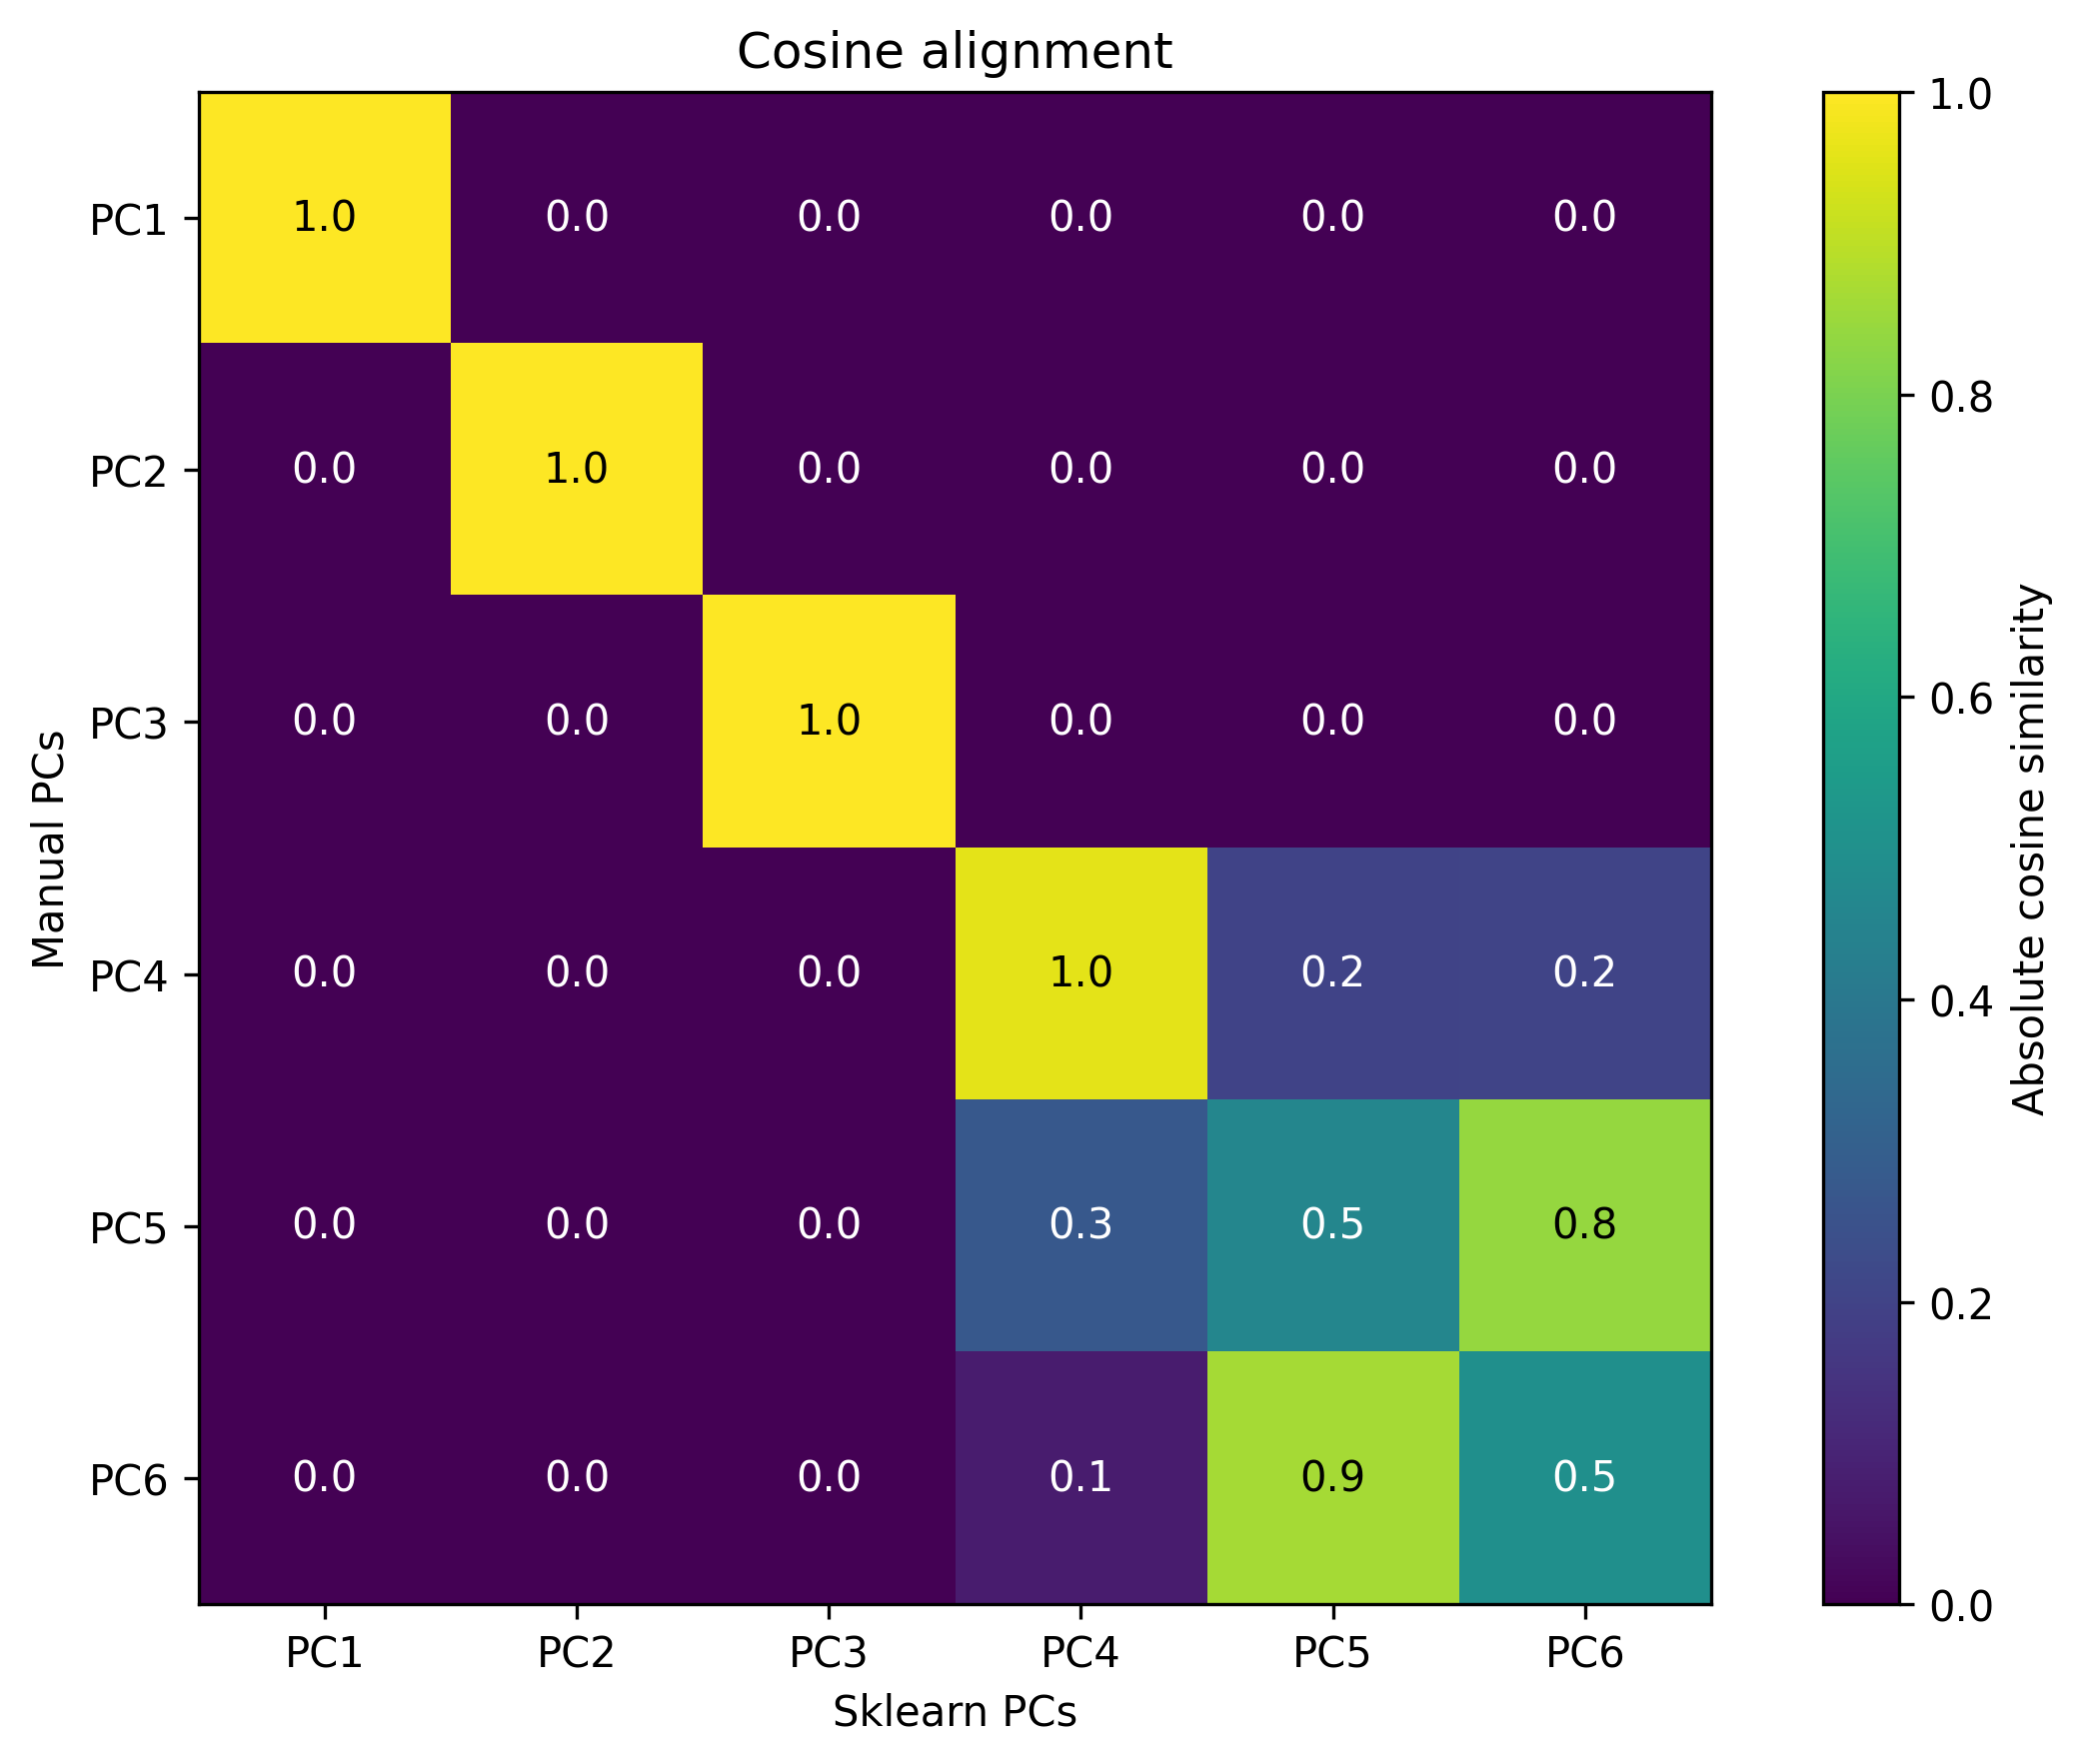
\includegraphics[width=\textwidth]{cosine_alignment.png}
\end{subfigure}
\hfill
\begin{subfigure}{0.24\textwidth}
    \centering
    \caption*{\textbf{D}}
    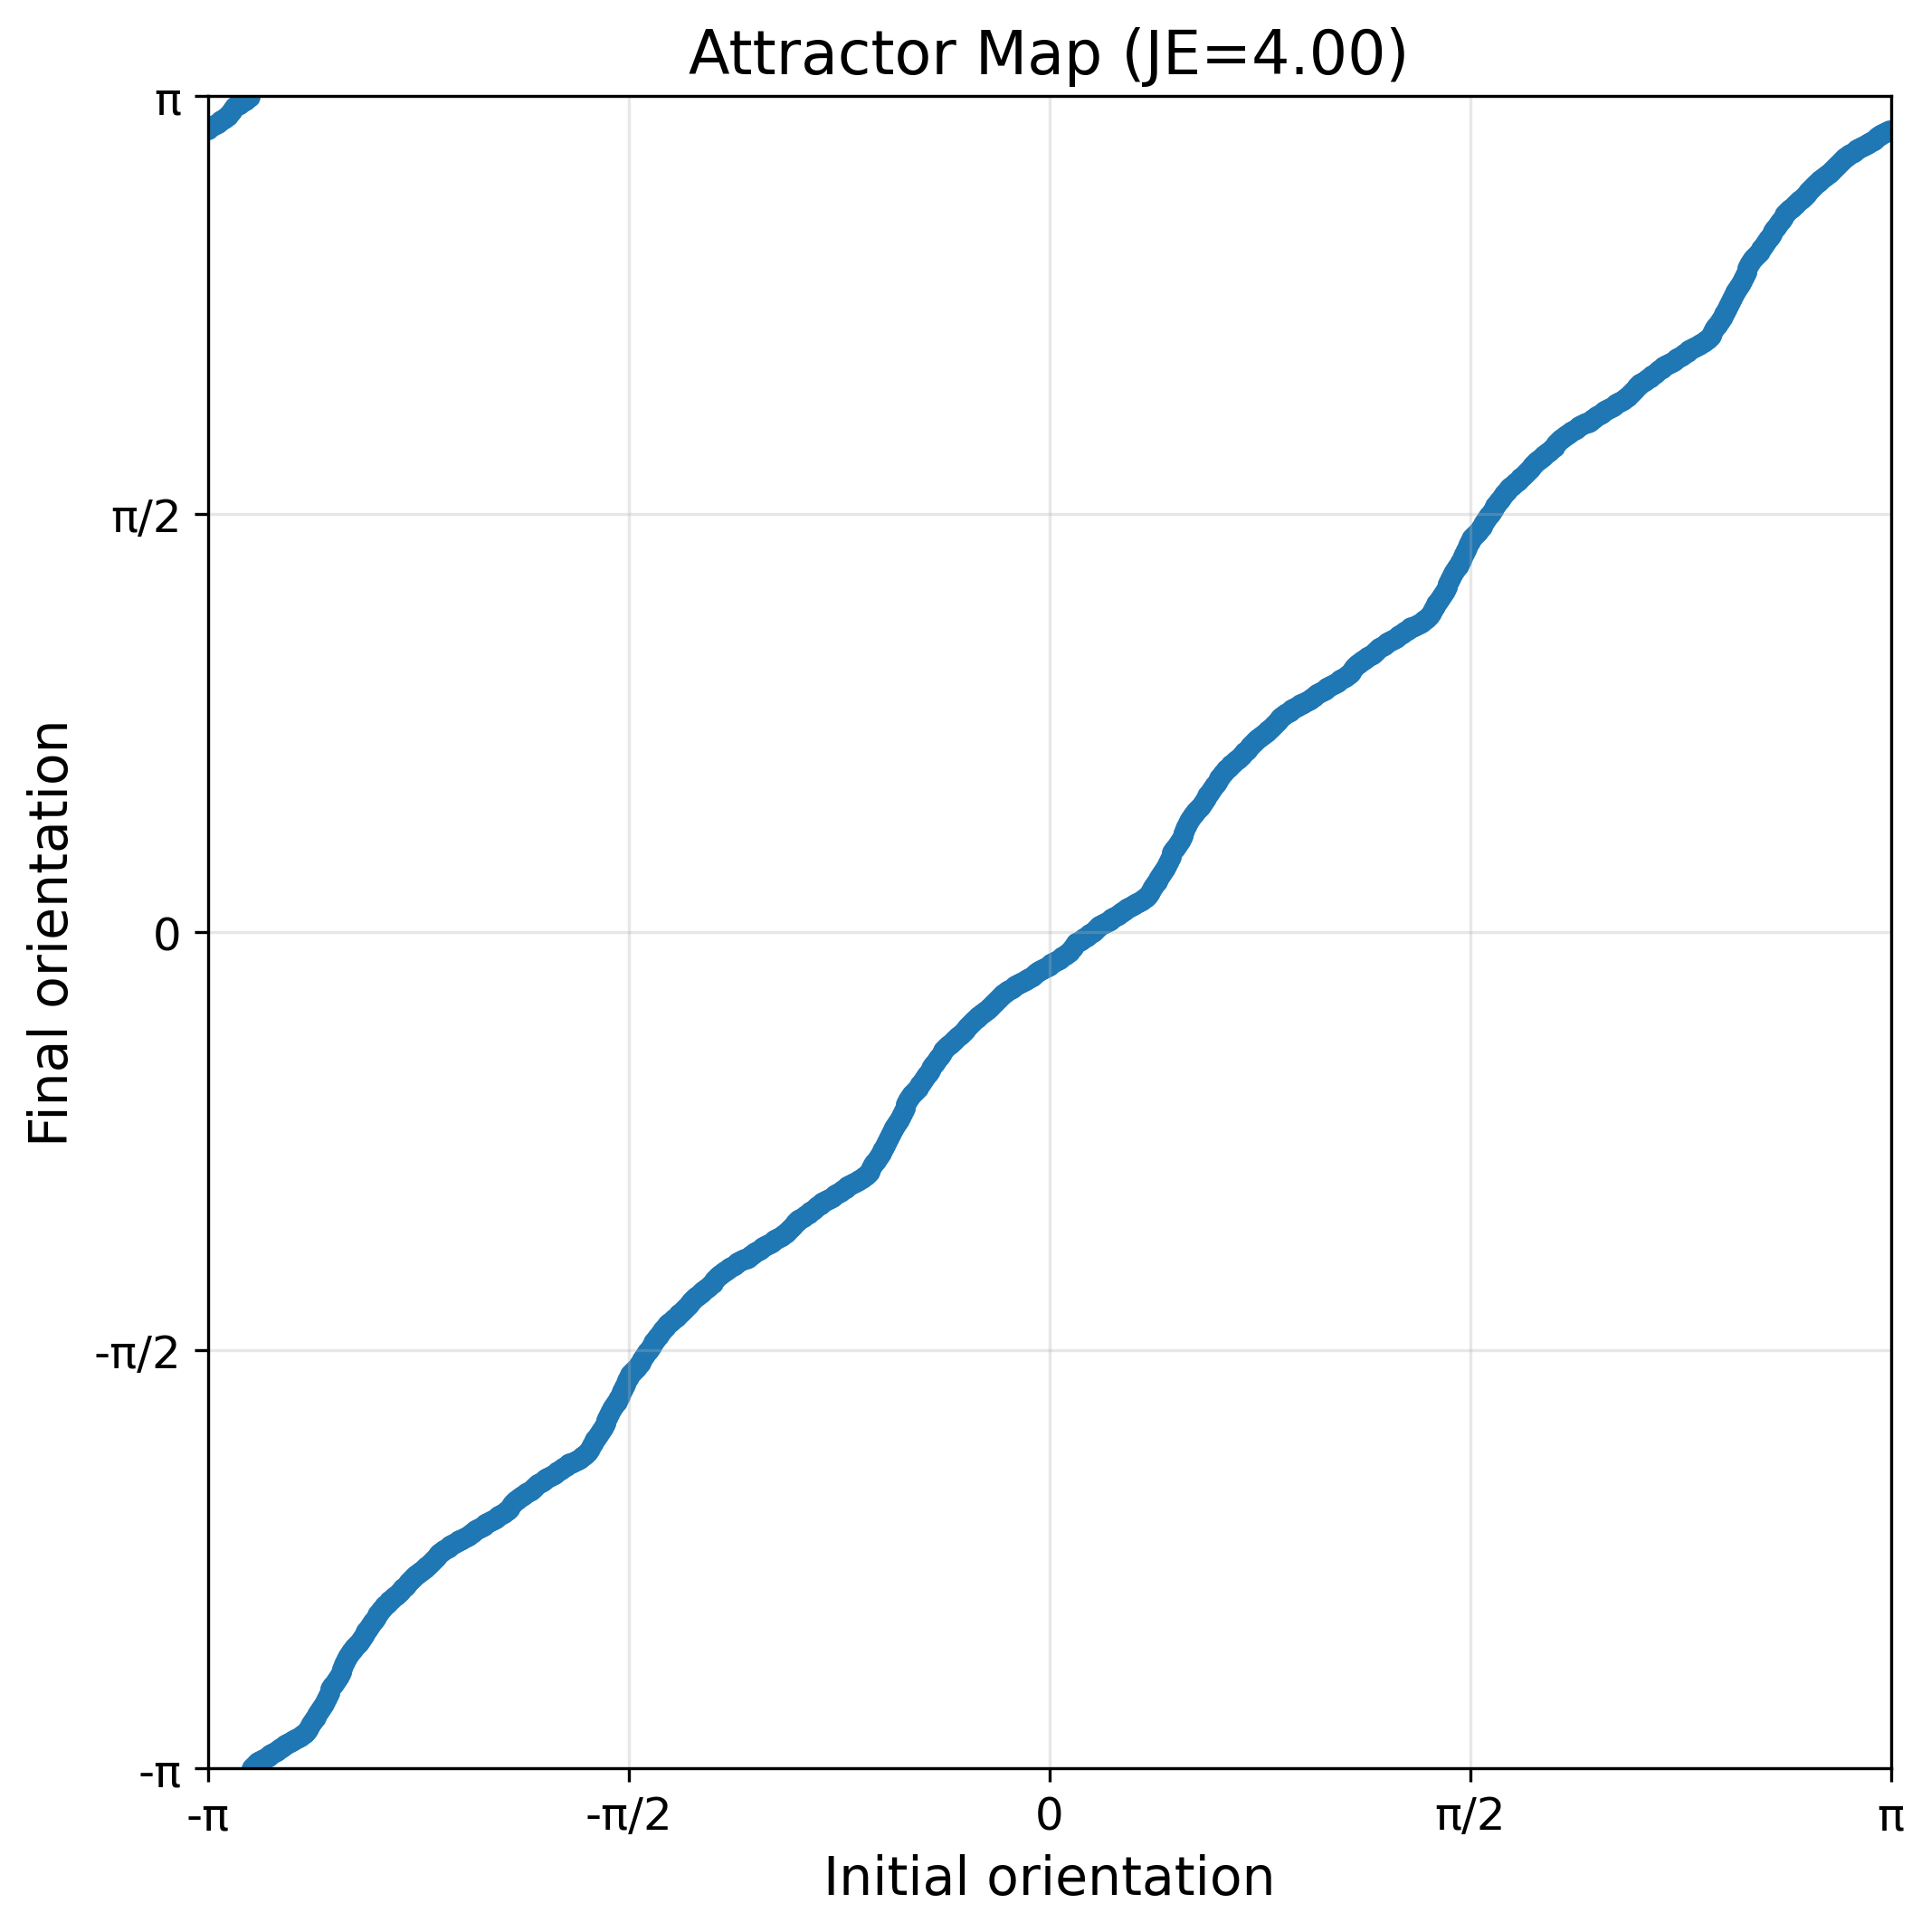
\includegraphics[width=\textwidth]{orientation_comparison.png}
\end{subfigure}

\caption{PCA analysis of ring attractor network dynamics. (A,B) Both manual and scikit-learn PCA implementations reveal a circular manifold in the first two principal components, indicating a continuous ring attractor. (C) The cosine alignment between methods confirms implementation correctness. (D) The network maintains all orientations without discretizing, demonstrating true continuous attractor dynamics.}
\label{fig:pca_analysis}
\end{figure}


\subsection{Influence of Different Parameter Sets}

\subsubsection*{Effect of \( J_E \) on Network Dynamics Without Angular Velocity Input}

To examine how synaptic tuning shapes network stability, we varied the local excitation strength \( J_E \) across six values used in Fig.~2e of Noorman et al.: \( J_E \in \{12, 6, 4, 3, 2.4, 1.2\} \), with broad inhibition fixed at \( J_I = -2 \) and a constant feedforward drive of \( c_{\text{ff}} = 1 \) (Fig 3). 
These span a range from under- to over-excitation relative to the analytically derived optima \( J_E^\ast \) (2.4, 4, 12) for continuous attractors in a six-neuron ring network.

The network exhibits three qualitatively distinct regimes. At the extremes—\( J_E = 12 \) (strong excitation) and \( J_E = 1.2 \) (weak excitation)—the bump of activity remains unstable, failing to converge to a fixed orientation or maintain a coherent representation. 
% Instead, the dynamics drift or fluctuate persistently, indicating a breakdown of attractor structure.

Intermediate excitation strengths yield more robust behavior. At \( J_E = 6 \) and \( J_E = 3 \), activity eventually collapses onto a small set of discrete orientations, consistent with the presence of multiple point attractors. The network relaxes to isolated fixed points in state space, forming a fragmented representation of angular position.

Strikingly, at two finely tuned values, \( J_E = 4 \) and \( J_E = 2.4 \), the network maintains a nearly continuous representation: activity traces out a smooth, ring-shaped manifold in the first two principal components, with six-fold symmetry reflecting the network’s architecture. Although minor discontinuities are present due to finite-size sampling, the overall structure is consistent with a continuous attractor.

These results reveal a phase transition, only near optimal excitation strengths does the network support a stable continuum of head-direction states. Deviations from these values lead to either discrete attractors or complete instability, highlighting the critical role of recurrent tuning in sustaining a ring attractor without input.  
This result is particularly notable, as shown in the absence of angular velocity input, the network can sustain a continuum of heading representations over long durations—purely through recurrent dynamics—when the excitation strength is appropriately tuned. This demonstrates that, even without external drive, optimal synaptic parameters allow the network to maintain a stable ring attractor.

\begin{figure}[H]
\centering
\begin{subfigure}{\textwidth}
    \centering
    \caption*{\textbf{A}}
    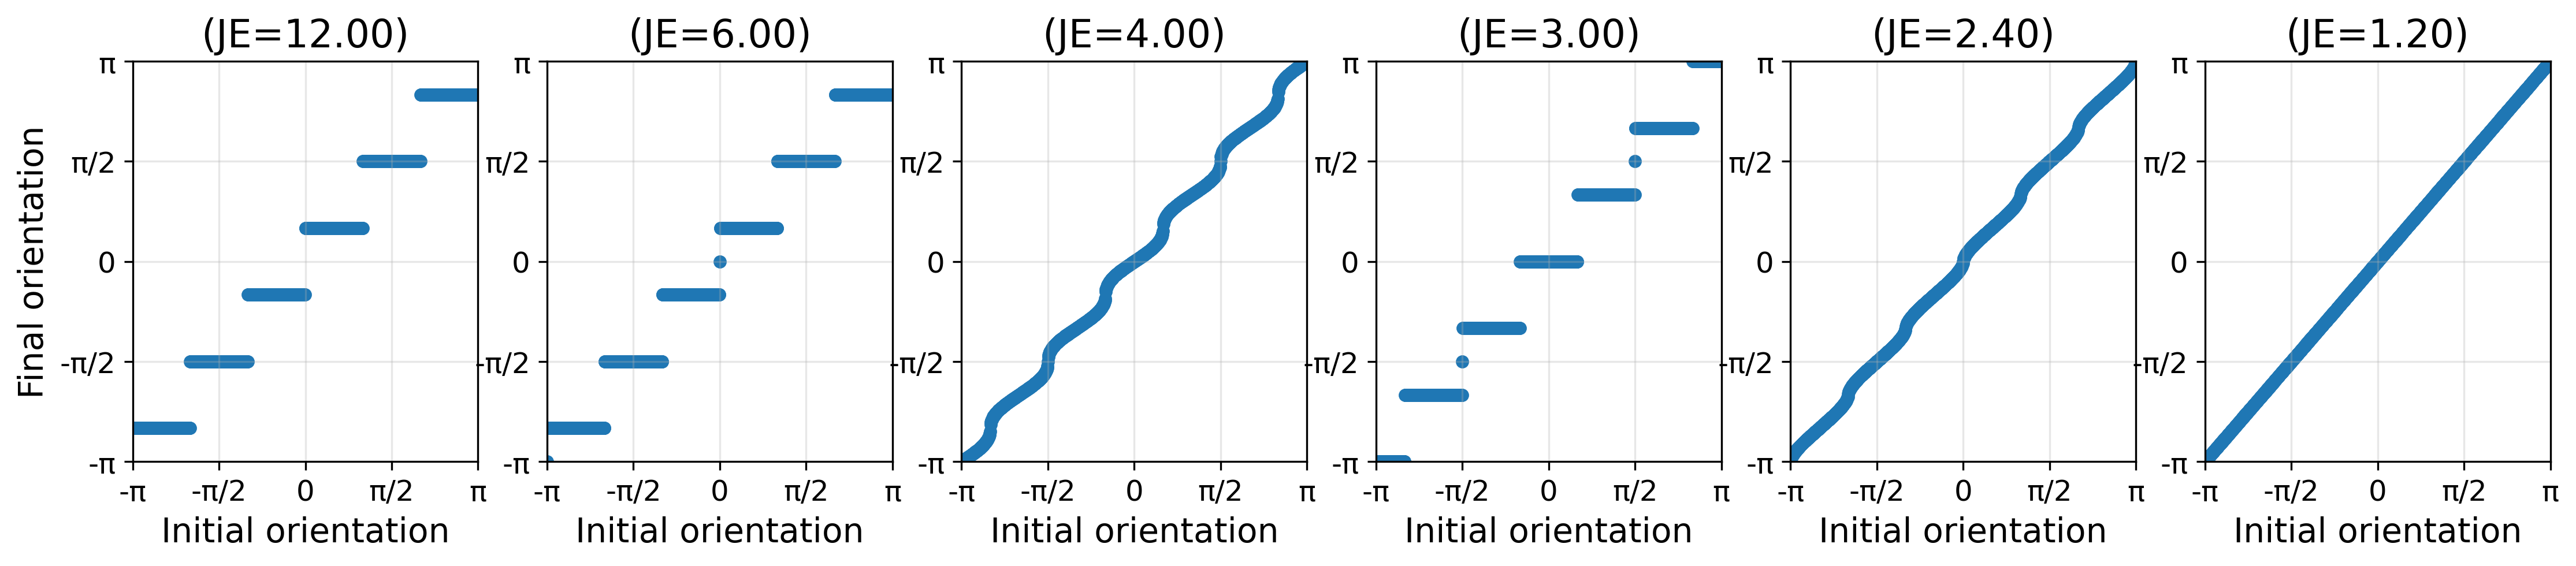
\includegraphics[width=\textwidth]{orientation_comparison_without_v.png}
\end{subfigure}

\vspace{0.1cm}

\begin{subfigure}{\textwidth}
    \centering
    \caption*{\textbf{B}}
    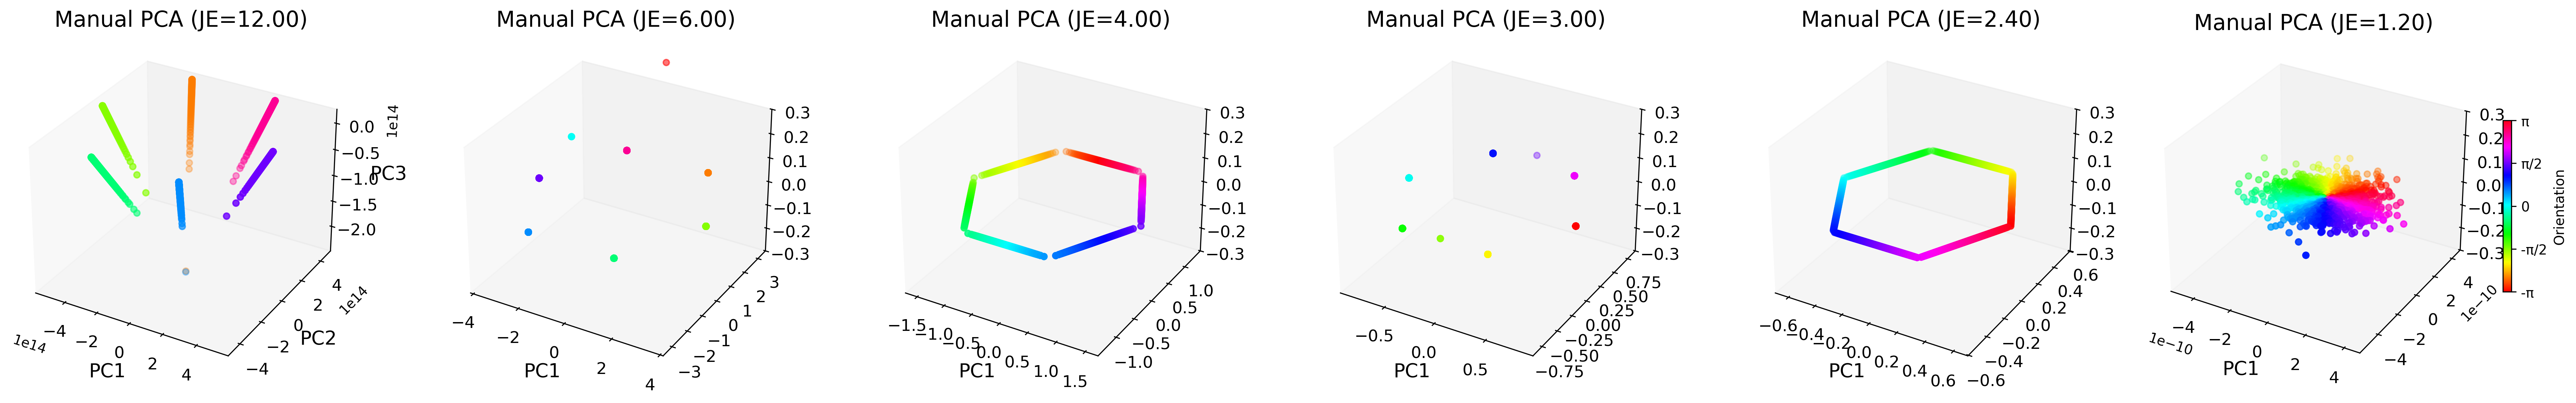
\includegraphics[width=1.0\textwidth]{manual_pca_without_v.png}
\end{subfigure}

\caption{Effect of excitation strength \( J_E \) on ring attractor dynamics. (A) Final vs. initial orientation for six different values of \( J_E \). Perfect diagonal relationships indicate continuous attractor behavior, while discrete clusters points indicate breakdown of the ring manifold. 
(B) Corresponding 3D PCA representations showing the attractor manifold structure. Smooth ring-like trajectories emerge at optimal \( J_E \) values (4.0 and 2.4), while other parameter settings produce either discrete point attractors or non-rubust dynamics.}
\label{fig:je_parameter_sweep}
\end{figure}



\subsubsection*{Effect of \( J_E \) on Network Dynamics with Angular Velocity Input}

To test how external drive interacts with synaptic tuning, we repeated the above analysis while introducing a constant angular velocity input \( v_{\text{in}} = 1.5 \) (Fig 4). This biases the bump’s motion along the ring, simulating continuous rotation. Unlike the previous section, the network was initialized with zero-mean Gaussian noise (standard deviation 0.1) rather than a pre-formed bump, to prevent the initial condition from favoring specific orientations.

As before, the two extremes of excitation (\( J_E = 12 \) and \( J_E = 1.2 \)) produce unstable dynamics: the bump fails to organize or follow the input in a coherent manner. In contrast, for intermediate \( J_E \), the bump evolves stably along the ring manifold, tracking the angular velocity.

Interestingly, within this regime, decreasing \( J_E \) leads to smoother ring attractors: the amplitude of the ups and downs in activity becomes more uniform, suggesting a flatter attractor landscape. This smoothness indicates that lower excitation—within a viable range—may enhance the network’s ability to continuously encode angular position during motion, potentially improving decoding accuracy.

These findings confirm that angular velocity inputs can effectively drive bump motion across the ring manifold, with optimal excitation strengths producing the most stable and continuous trajectories. The improved smoothness at moderate \( J_E \) values suggests that external drive can compensate for some discretization effects, enabling continuous integration even when the network is not perfectly tuned.

\begin{figure}[H]
\centering
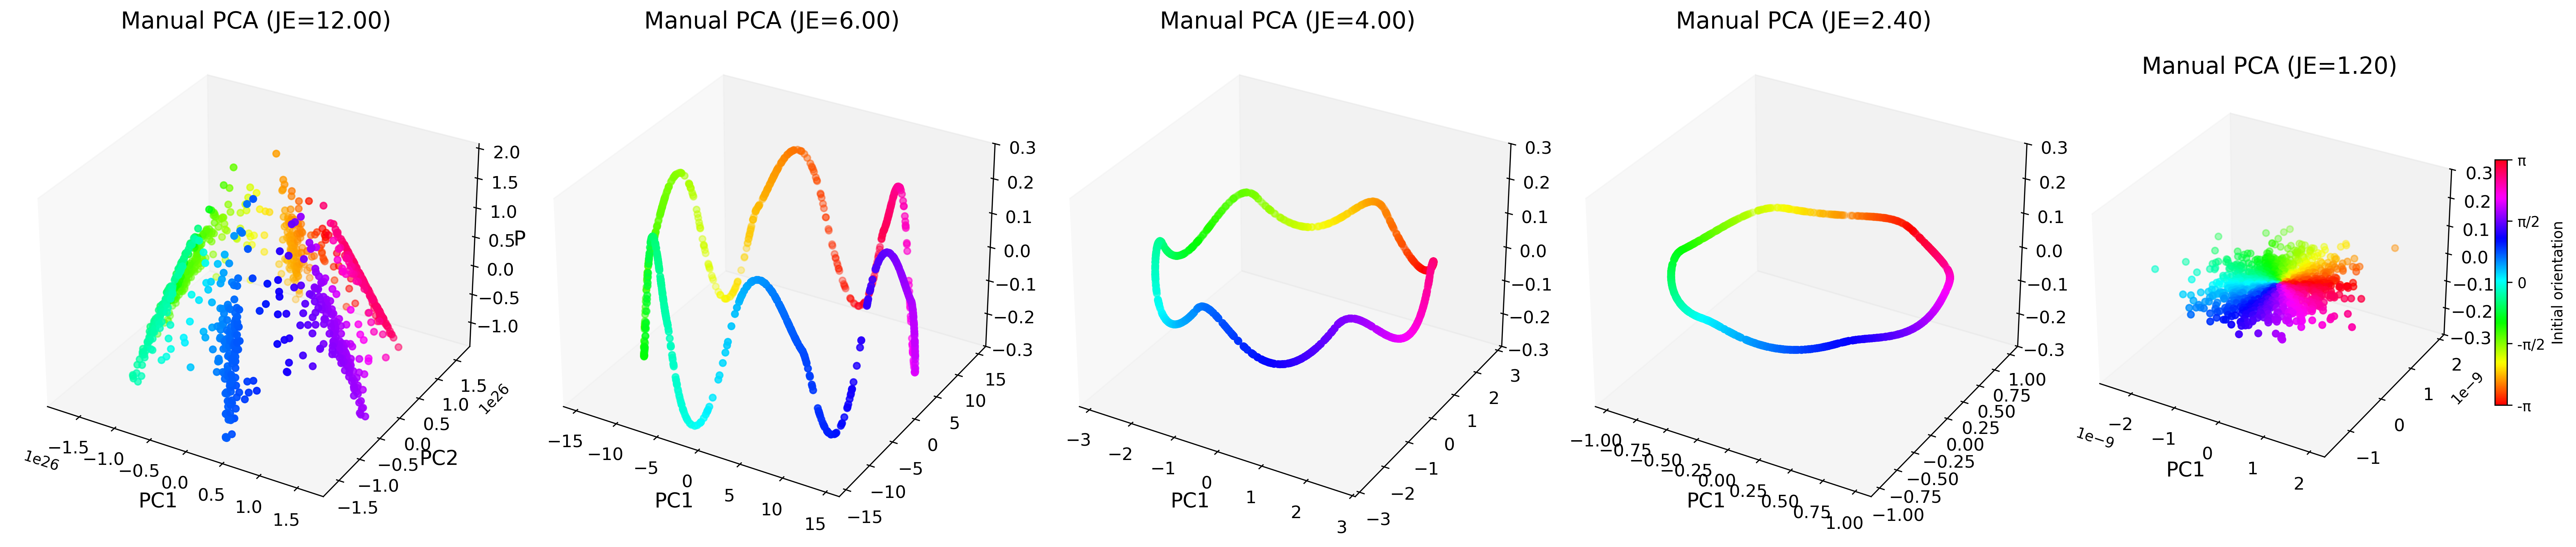
\includegraphics[width=1.0\textwidth]{manual_pca_with_v.png}
\caption{PCA analysis of ring attractor dynamics with angular velocity input (\( v_{\text{in}} = 1.5 \)). The 3D visualization shows how different excitation strengths \( J_E \) affect the attractor manifold when driven by external velocity. Smooth helical or ring-like trajectories indicate stable velocity integration, while irregular patterns suggest breakdown of continuous dynamics.}
\label{fig:pca_with_velocity}
\end{figure}


\subsubsection*{Effect of Feedforward Input (\( c_{\text{ff}} \)) on Network Dynamics with Angular Velocity Input}
To assess the role of feedforward input, we removed it by setting \( c_{\text{ff}} = 0 \) while keeping the angular drive active (\( v_{\text{in}} = 1.5 \)). 
We then varied the local excitation strength across three moderate values: \( J_E \in \{7.0, 4.0, 3.0\} \). 
Unlike the previous conditions where feedforward input was present, the network no longer forms a coherent ring structure in the low-dimensional activity space (Figure 5). 
Instead, the population activity appears as a diffuse cloud lacking any clear manifold geometry.

While some separation by head-direction angles remains—indicating that directional information is partially retained—the encoding is unstable. 
The same head-direction angles can correspond to multiple, inconsistent positions in state space, undermining reliable decoding. 
These results highlight the importance of feedforward input in stabilizing the bump’s position and preserving consistent head-direction representations across trials.

\begin{figure}[H]
\centering
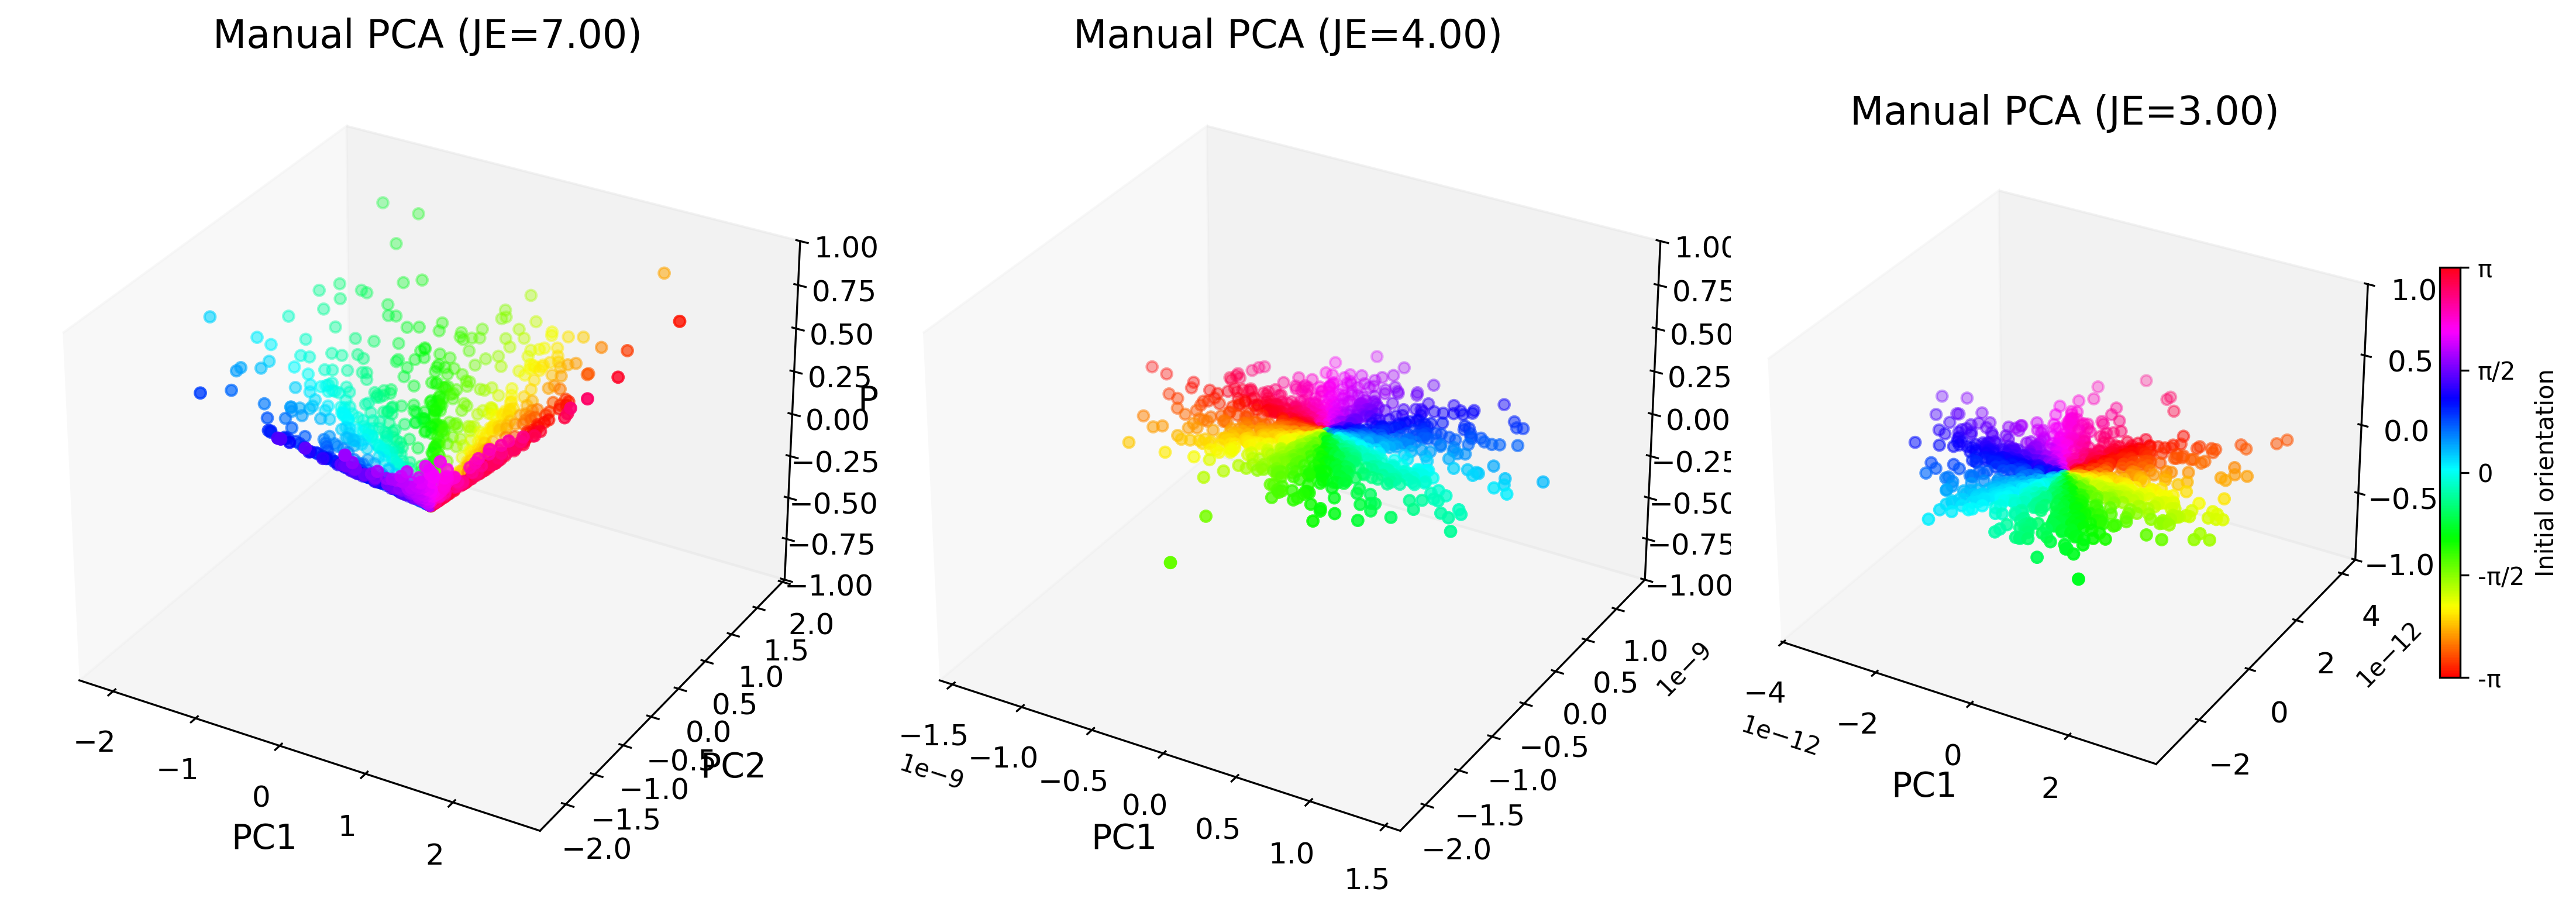
\includegraphics[width=1.0\textwidth]{manual_pca_cff_zero.png}
\caption{PCA analysis of ring attractor dynamics without feedforward input (\( c_{\text{ff}} = 0 \)). Without constant feedforward drive, the network fails to maintain a coherent ring manifold structure across different excitation strengths \( J_E \). The population activity forms diffuse clouds rather than organized trajectories, indicating non-robust encoding despite preserved directional sensitivity.}
\label{fig:pca_cff_zero}
\end{figure}


\subsubsection*{Effect of Number of neurons on Network Dynamics}
We also investigated the no-input condition (\( v_{\text{in}} = 0 \)) in a larger network with 100 neurons, keeping the feedforward input fixed at \( c_{\text{ff}} = 1 \). Like smaller networks, extreme values of \( J_E \) still induce phase transitions that disrupt stable head-direction encoding. Whereas the smaller network required fine-tuned parameters to sustain a continuous ring attractor, the larger network reliably supports continuous encoding across all intermediate \( J_E \) values. This behavior is shown in Figure 6 , where the latent activity organizes into a well-defined ring manifold despite the absence of input.

% The increased robustness stems from the greater redundancy and higher representational capacity afforded by the larger network. With more neurons, the system can tolerate minor variations in the bump’s shape or position, enabling stable continuous attractor dynamics without requiring precise tuning of synaptic parameters.

\begin{figure}[H]
\centering
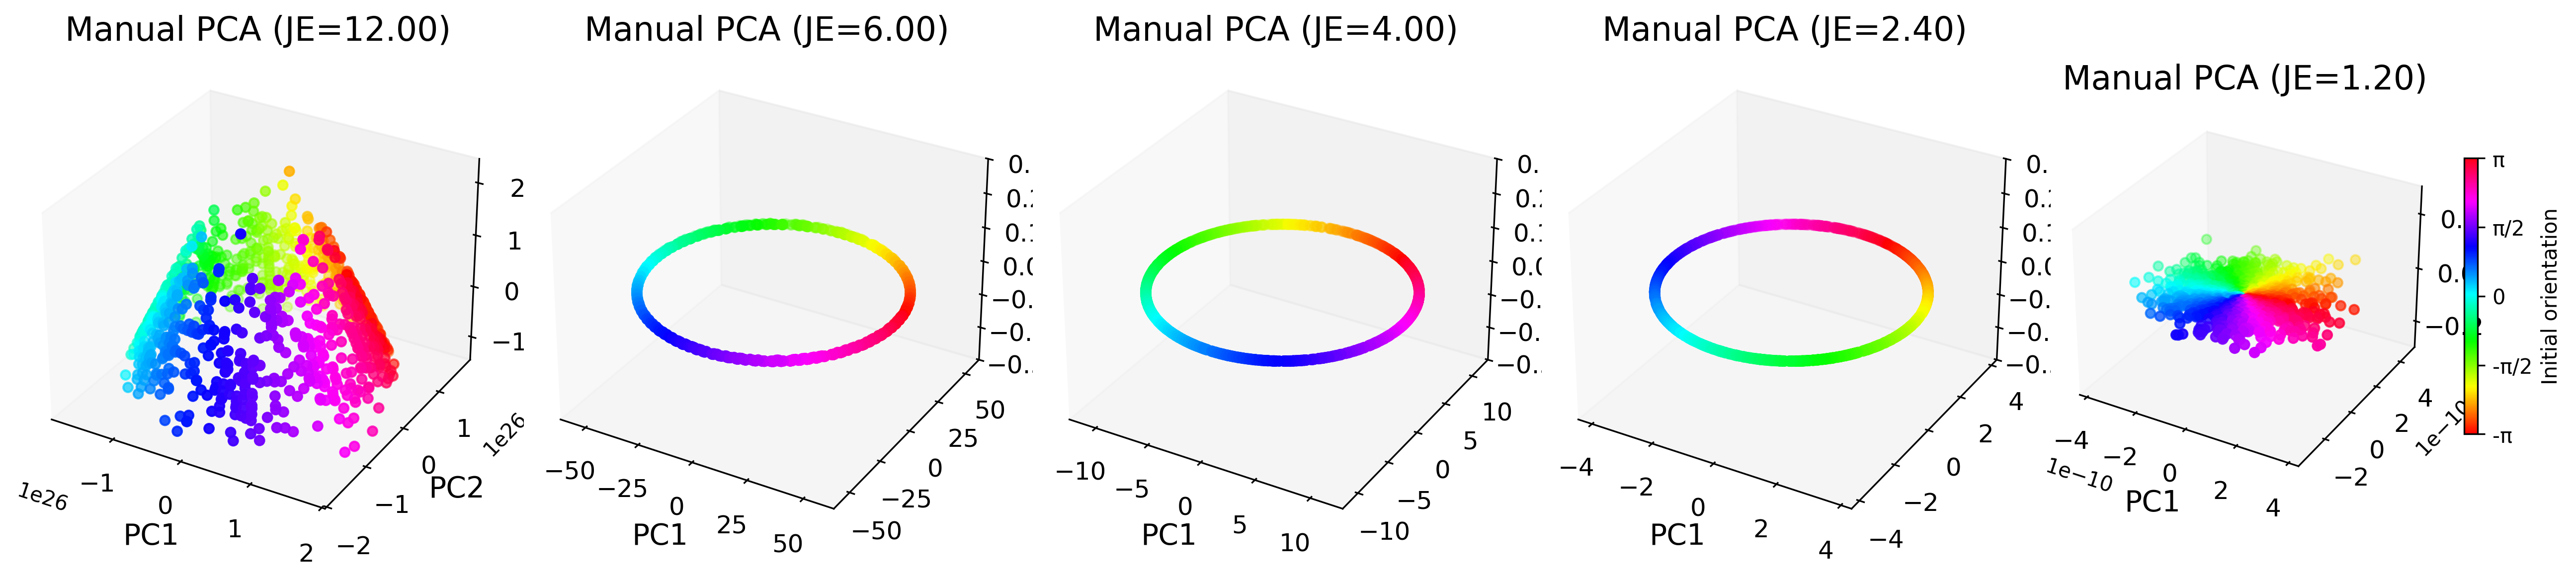
\includegraphics[width=1.0\textwidth]{manual_pca_large_network.png}
\caption{PCA analysis of ring attractor dynamics in a 100-neuron network without angular velocity input (\( v_{\text{in}} = 0 \)). The larger network maintains robust ring manifold structure across all intermediate excitation strengths \( J_E \), demonstrating increased stability and continuous encoding compared to smaller networks. The smooth circular trajectories indicate that larger networks are less sensitive to parameter tuning while preserving continuous attractor dynamics.}
\label{fig:pca_100_neurons}
\end{figure}


\subsection*{Effect of Network Size on Attractor Manifold Dimensionality}

We examine how the dimensionality of the network's activity changes with the number of neurons, varying $N$ from 4 to 100. To investigate this systematically, we consider two parameter regimes that highlight different aspects of the size-dependent behavior.

\subsubsection*{Optimal Excitation: Sparse Sampling of a Continuous Ring}

First, we fix the network parameters to $J_I = -2$, $J_E = 4.0$, $v_{\text{in}} = 0$, and $c_{\text{ff}} = 1$. With the recurrent excitation weight tuned to the optimum $J_E \approx 4$, the network implements a true continuous ring attractor—even when it contains only four head-direction cells (Fig 7). 

Principal component analysis (after mean-centering) consistently identifies the same two principal axes that correspond to the Fourier pair $(\cos\psi, \sin\psi)$; the third component carries virtually no variance. For very small $N$, the continuous manifold is merely \emph{sparsely sampled}, so its projection appears as a square ($N=4$) or hexagon ($N=6$) in the $\text{PC}_1$–$\text{PC}_2$ plane. Adding neurons simply inserts intermediate sample points, transforming the polygon into an increasingly smooth circle. Importantly, nothing changes topologically or dimensionally: the steady-state activity always lies on a one-dimensional ring embedded in a two-dimensional subspace. The apparent "square $\to$ ring" progression is purely a resolution effect, not a transition from discrete to continuous dynamics.

\begin{figure}[H]
\centering
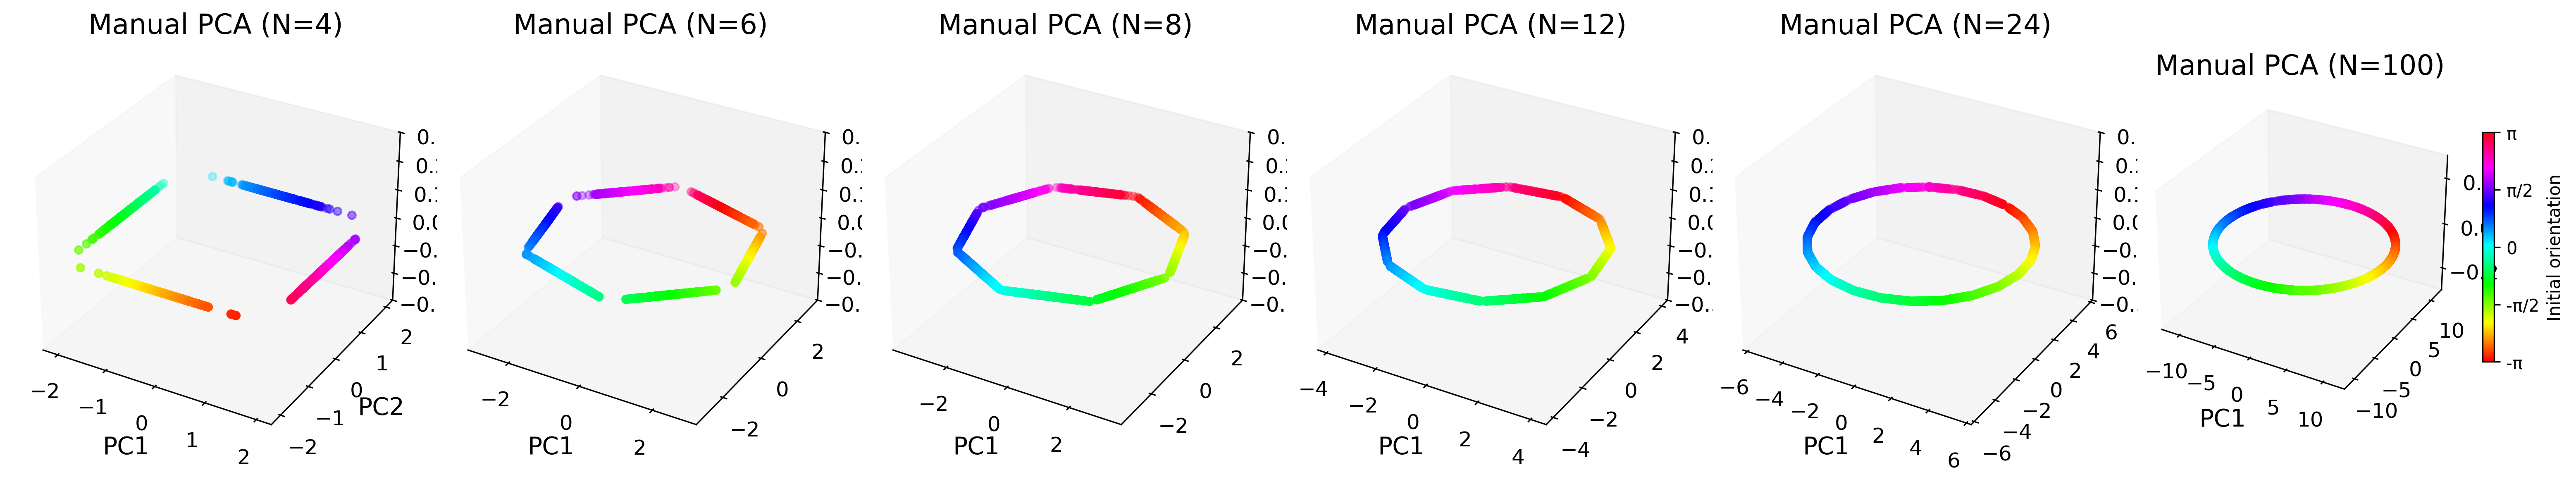
\includegraphics[width=1.0\textwidth]{manual_pca_varying_N_ring.png}
\caption{PCA analysis of ring attractor dynamics across network sizes with optimal excitation ($J_E = 4.0$). From left to right: $N = 4, 6, 8, 12, 24, 100$ neurons. The continuous ring manifold is preserved at all sizes, with smaller networks showing sparse sampling (polygonal appearance) that becomes increasingly smooth as more neurons are added. The underlying topology remains unchanged—a one-dimensional ring embedded in two-dimensional space.}
\label{fig:network_size_optimal}
\end{figure}

\subsubsection*{Elevated Excitation: Discrete-to-Continuous Transition}

Next, we increase the excitatory weight slightly above the sweet-spot, setting $J_I = -2$, $J_E = 5.0$, $v_{\text{in}} = 0$, and $c_{\text{ff}} = 1$ (Fig 8). This elevated excitation makes the activity bump "too strong," creating an uneven energy landscape where not every heading is equally stable for the network.

With only a few neurons ($N = 4$ or $6$), the bump can settle stably at just a handful of preferred directions, so the PCA plots show \textbf{isolated clusters} instead of a continuous manifold. Some initial conditions still converge toward ring-like trajectories, resulting in a mixture of discrete points and partial ring segments. As we increase the number of neurons, the possible stable headings become more finely spaced; the isolated clusters gradually fill in the gaps, and by $N \approx 24$, the representation resembles a \textbf{smooth ring} again. 

This demonstrates that $J_E = 5$ fragments the ring into discrete "islands" for small networks, but the continuous ring re-emerges once the network is large enough to resolve finer angular increments. Unlike the optimal case, this represents a genuine discrete-to-continuous transition driven by network size.

\begin{figure}[H]
\centering
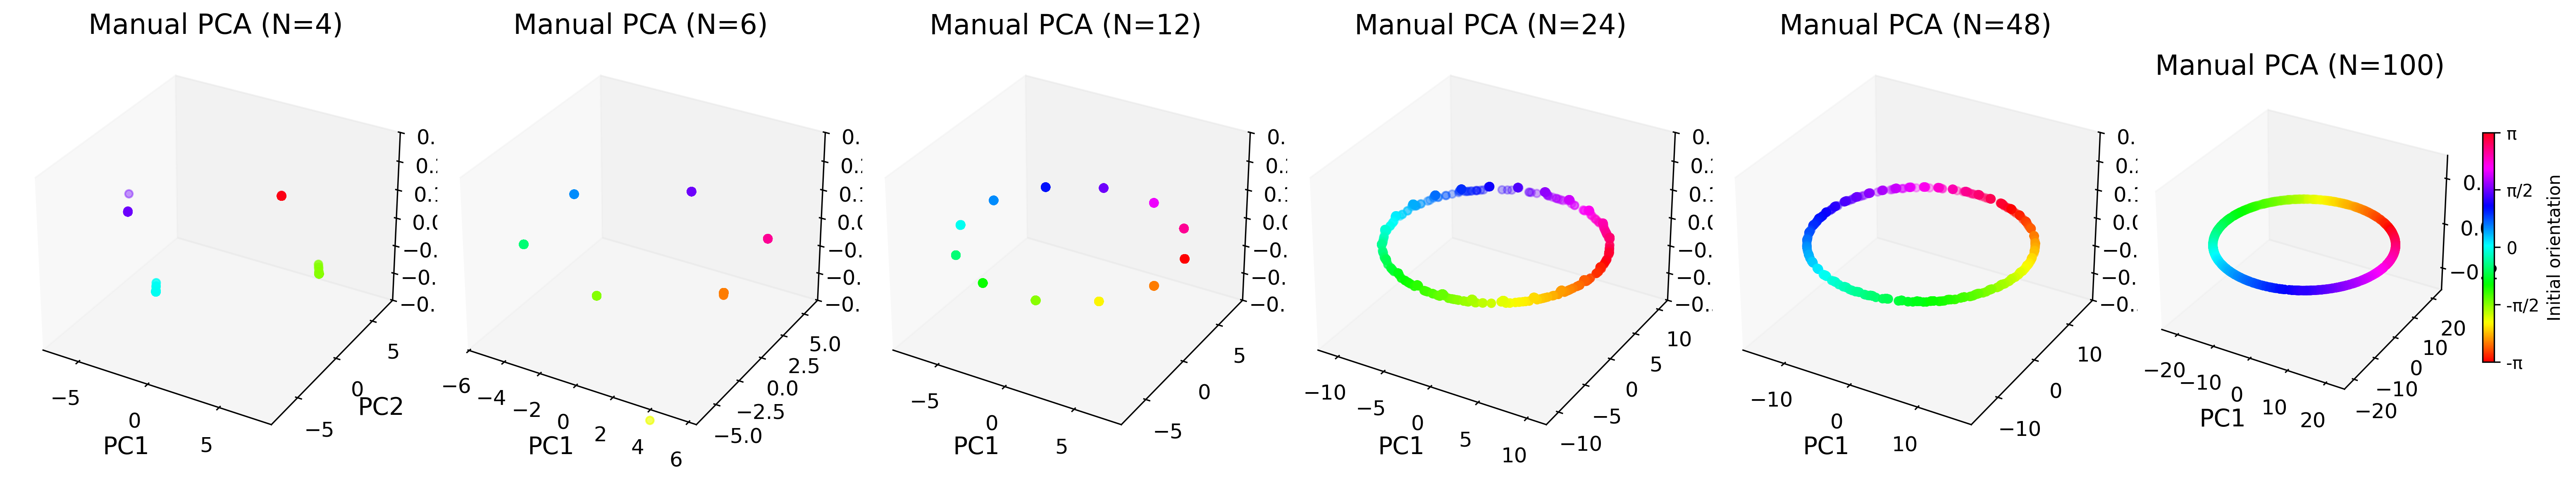
\includegraphics[width=1.0\textwidth]{manual_pca_varying_N_point.png}
\caption{PCA analysis of ring attractor dynamics across network sizes with elevated excitation ($J_E = 5.0$). From left to right: $N = 4, 6, 12, 24, 48, 100$ neurons. Small networks exhibit discrete point attractors (isolated clusters), while larger networks recover continuous ring dynamics. This represents a genuine discrete-to-continuous transition as network size increases, unlike the sparse sampling effect observed at optimal excitation.}
\label{fig:network_size_elevated}
\end{figure}


\subsection{Stability Restults}

Noorman et al. analyze the stability of a small ring attractor network using a dynamical systems approach, showing that continuous representations of circular variables, like head direction, can be maintained with as few as four neurons. This is achieved by constructing a set of line attractors, each defined by a fixed subset of active neurons, and smoothly transitioning between them as the bump of activity shifts. These stitched-together line attractors form a continuous ring attractor manifold. The bump configuration is characterized by its amplitude \( a \), width \( w \), and orientation \( \psi \), and the dynamics reduce to three differential equations governing how these evolve over time. A fixed point, representing a stable bump, occurs when all three derivatives vanish. Crucially, the stability of these fixed points depends on whether perturbations in bump orientation decay (\( \lambda_\psi < 0 \)) or are neutrally stable (\( \lambda_\psi = 0 \)). The system achieves marginal stability (a continuous attractor) when the strength of local excitation \( J_E \) is tuned to an optimal value \( J_E^* \), satisfying:
\begin{equation}
\frac{1}{J_E^*} = \frac{1}{N} \sum_{k \in K_{\text{act}}} \sin^2(\theta_k - \psi^*)
\end{equation}

This ensures the curvature of the energy landscape is flattened along the ring, enabling drift-free persistent activity.

When the network is optimally tuned in this way, narrow and robust bumps form that do not drift in the absence of input, allowing the network to stably represent continuous angular variables. Perturbations orthogonal to the attractor manifold (i.e., changes in bump width or amplitude) are suppressed due to negative eigenvalues, while motion along the attractor (changes in \( \psi \)) is marginally stable. This tuning balances local excitation with global inhibition and ensures that the active submatrix of the recurrent connectivity has a zero leading eigenvalue, an indicator of line attractor dynamics. If \( J_E \) deviates from its optimal value, the bump either drifts toward discrete fixed points or becomes unstable. Thus, the network’s ability to maintain continuous attractor dynamics, and hence a faithful internal representation of variables like head direction, depends critically on fine-tuned parameters that place it near the boundary between stability and marginal stability.


\subsection{Summary of Figure 2 (Noorman \emph{et al.})}

Figure 2 demonstrates that even a very small head-direction ring network can sustain a continuous “bump’’ of activity when analysed through an energy‐landscape framework.  \(N\) neurons are arranged around a circle with short-range excitation (\(J_E\)) superimposed on broad inhibition (\(J_I\)), and the authors derive an energy functional \(E(a,w,\psi)\) whose minima correspond to stationary bumps parametrised by amplitude \(a\), width \(w\) and orientation \(\psi\).  With arbitrary parameters the energy surface is corrugated along \(\psi\), so the bump is pinned to a few discrete headings, turning the circuit into a finite set of point attractors.

The study then identifies a family of "sweet-spot" excitation strengths \(J_E^{\!*}(N_{\text{act}})\) (one for every admissible number of active neurons) that null the orientation curvature \(\partial^{2}E/\partial\psi^{2}\).  At any such optimum the \(\psi\)-direction becomes \emph{flat}, producing a continuum of marginally stable bump states: numerical simulations exhibit zero drift in darkness, linear response to infinitesimal velocity inputs, and an active-sub-matrix with a single zero eigenvalue.  Hence, a ring comprising as few as four to six neurons can emulate an ideal ring attractor—provided local excitation is tuned to one of these optima.

Detuning \(J_E\) above or below its optimal value re-introduces curvature, breaking the flat ridge into alternating minima and saddles.  The bump then drifts toward the nearest minimum, ignores inputs below a threshold, and accelerates or decelerates as it crosses successive ridges under stronger drive; drift rate, threshold velocity and integration linearity all scale with \(|J_E-J_E^{\!*}|\).  Figure 2 thus makes the case that precise, yet biologically plausible, tuning of local excitation is both necessary and sufficient for a tiny discrete network to function as a continuous ring attractor, while even mild mistuning resurrects the classic finite-size failure modes.

\section{Conclusion}

Our computational investigation provides strong support for the theoretical framework proposed by Noorman et al. (2024), demonstrating that small ring attractor networks can indeed maintain continuous representations when optimally tuned. 
Through systematic PCA analysis across different parameter regimes and network sizes, we validated several key predictions about the relationship between excitation strength and attractor manifold structure.

The PCA revealed the geometry of the attractor manifold: when the network supports a continuous ring attractor, the final states trace a smooth circular trajectory in principal component space; in contrast, discretized networks exhibit distinct clusters corresponding to stable point attractors. This geometric perspective provides direct visual evidence for the theoretical distinction between continuous and discrete attractor regimes.

Key findings include:
\begin{itemize}
\item Optimal excitation tuning (\(J_E = 4.0\) and \(J_E = 2.4\)) produces smooth ring manifolds in 6-neuron networks, confirming the existence of "sweet spot" values that eliminate orientation curvature
\item Deviations from optimal \(J_E\) systematically degrade continuous representation, either creating discrete point attractors (intermediate values) or unstable dynamics (extreme values)
\item Network size effects reveal that larger networks (N=100) maintain continuous attractors across broader parameter ranges, while smaller networks require precise tuning—consistent with the theoretical prediction that discretization sensitivity scales inversely with network size
\item External velocity inputs can drive smooth bump motion along the ring manifold when excitation is appropriately tuned, validating the networks' capacity for angular velocity integration
\item Feedforward input (\(c_{\text{ff}}\)) is essential for maintaining stable bump positioning and consistent directional encoding
\end{itemize}

These results demonstrate that the PCA-based geometric analysis provides powerful additional support for the authors' central claims about excitation tuning in small continuous attractor networks. The clear correspondence between theoretical predictions and empirical manifold structure strengthens confidence in the biological plausibility of such minimal yet sophisticated neural circuits, with important implications for understanding navigation systems in compact brains like those of insects.


\begin{thebibliography}{9}

\bibitem{noorman2024}
Noorman, M., Hulse, B.K., Jayaraman, V. et al. 
Maintaining and updating accurate internal representations of continuous variables with a handful of neurons. 
\textit{Nat Neurosci} \textbf{27}, 2207–2217 (2024). 
\url{https://doi.org/10.1038/s41593-024-01766-5}

\bibitem{compte2000}
Compte, A., Brunel, N., Goldman-Rakic, P.S., Wang, X.-J.
Synaptic Mechanisms and Network Dynamics Underlying Spatial Working Memory in a Cortical Network Model.
\textit{Cerebral Cortex} \textbf{10}(9), 910–923 (2000).
\url{https://doi.org/10.1093/cercor/10.9.910}

\bibitem{zhang1996}
Zhang, K.
Representation of spatial orientation by the intrinsic dynamics of the head-direction cell ensemble: a theory.
\textit{Journal of Neuroscience} \textbf{16}(6), 2112-2126 (1996).
\url{https://doi.org/10.1523/JNEUROSCI.16-06-02112.1996}

\end{thebibliography}
\end{document}
